\chapter{Implementation}
\label{chap:implementation}

This section describes the artefact development process. Despite multiple stumbling blocks during development, these were overcome through problem-solving, thorough investigation and reading of software documentation.  

\section{Development Environment}
\label{implementation:de}

Visual Studio Code (VS Code) was chosen as the development environment for development (\cite{noauthor_visual_nodate}). VS Code was chosen due to its flexibility in working with multiple programming languages through the use of extensions. The React.js Framework, JavaScript and Go Language extensions were installed to ensure seamless development of the backend and frontend of the artefact. The ESLint extension was also used using Go and JavaScript configurations to ensure the consistency and readability of the codebase.

\section{Iteration 1 - Basic UI and Core Routing}
\label{implementation:iteration1}
The initial stages of development began using a first draft of elicited requirements \see{appendix:initial-user-requirements} where later in the project, a new set of user requirements was formed based on primary research. This method proved effective in not delaying initial development, where the core requirements were unlikely to change greatly. Furthermore, Iteration 1 consisted of implementing the building blocks of the artefact, including setting up a React.js App, Gin Webserver, PostgreSQL database and the core routing functionalities.

\subsection{Leaflet - Open Street Map (OSM)}
\label{iteration1:leaflet-osm}
The Map component was the first to be developed because the rest of the artefact would be dependent on its mapping functionality. The component contained a div element containing the MapContainer component imported from React Leaflet (\cite{noauthor_react_nodate}). The component includes a tile layer to make API requests to Open Street Map (\cite{noauthor_openstreetmap_nodate}) to get the tile images for the map, and then display these tiles to form the full-screen map element. Temporary variables were set up to store the latitude and longitude values representing the start and end of a route, then drawn on the map using a polyline and marker points \see{fig:basic-map-with-route}. 

\begin{figure}[!ht]
    \centering
    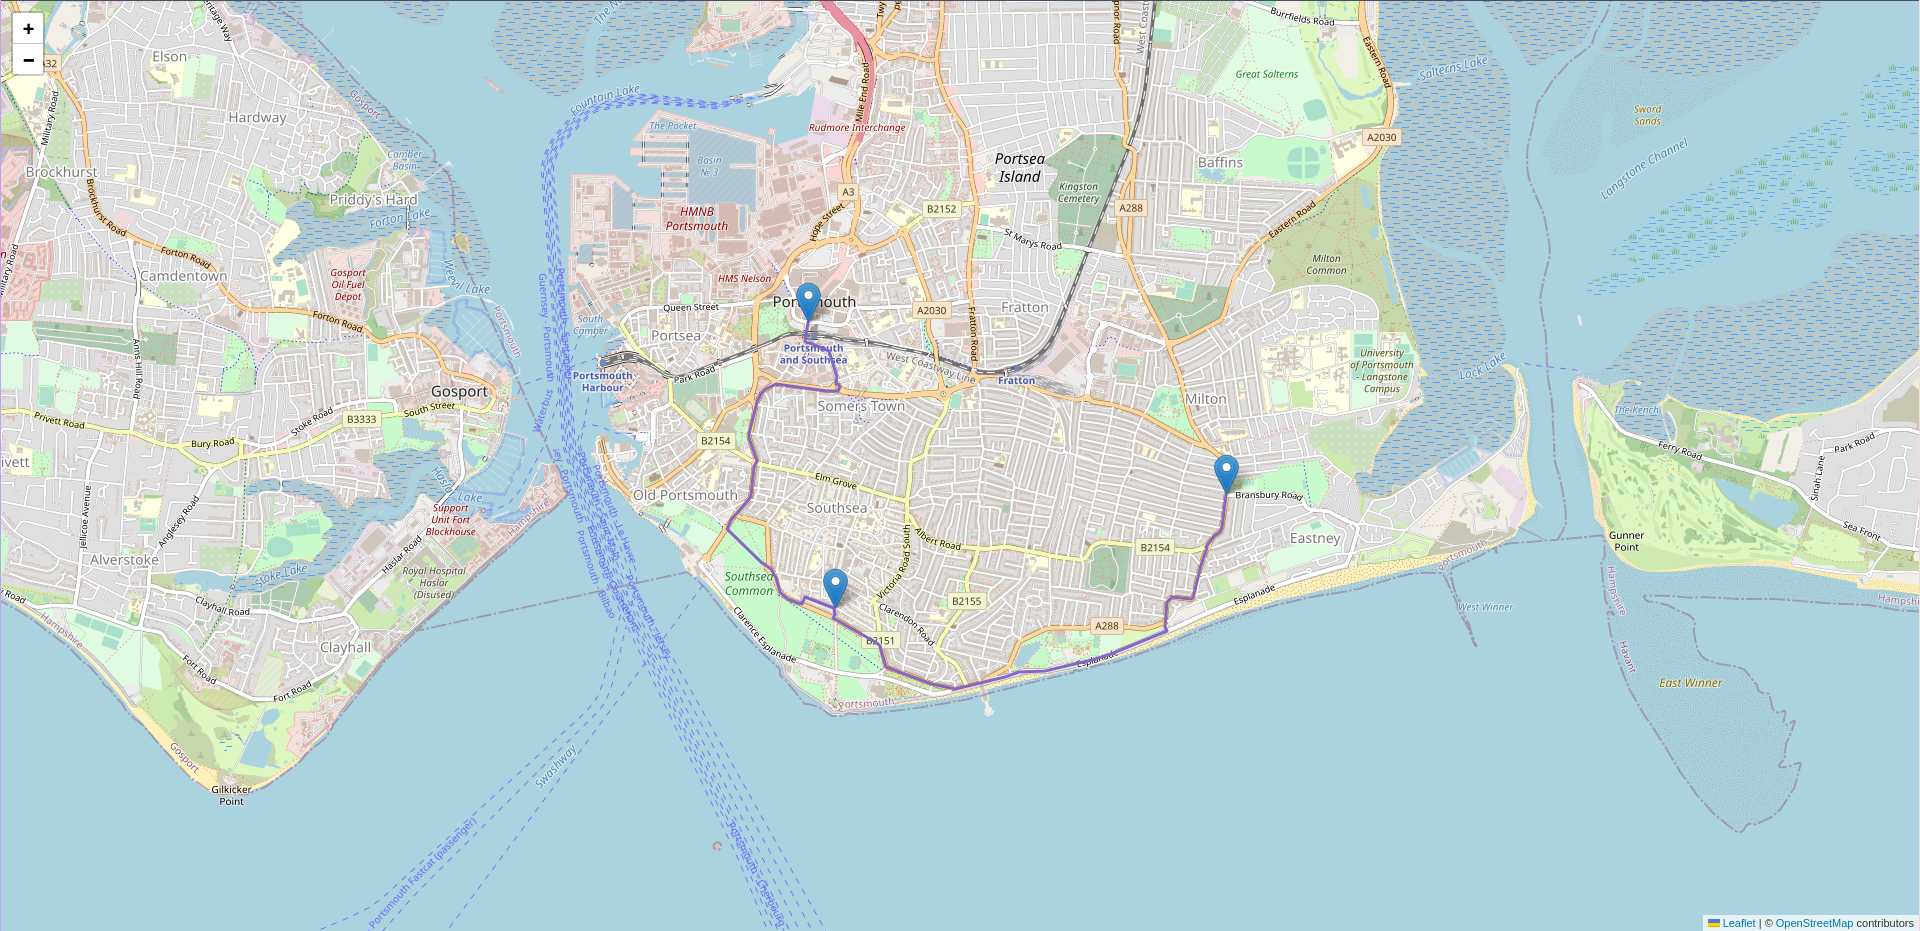
\includegraphics[width=425px]{figures/Progress Images/Iteration-1/SR25/Basic Route.png}
    \caption{Basic Map with Route}
    \label{fig:basic-map-with-route}
\end{figure}

\subsection{Basic Route Planning}
\label{iteration1:basic-routing}
After conducting research, the most effective way to implement route planning with Leaflet was to use Leaflet Routing Machine (\cite{noauthor_leaflet_nodate-1}). This library enabled a RoutingMachine component to be natively added on top of the React Leaflet map component, whilst providing a basic, customisable route planning UI \see{fig:routing-ui}. The routing API in use at the beginning was Open Source Routing Machine (OSRM) (\cite{noauthor_project_nodate}) which appeared to meet all requirements of a routing algorithm until round trip routing was required \see{iteration3:round-trip}. This new routing functionality enabled the user to select a start, destination and any intermediate locations, a route would then be planned. At this stage, the route could be altered through the use of waypoints, but the artefact did not provide any further custom routing features to the user.
\begin{figure}[!ht]
    \centering
    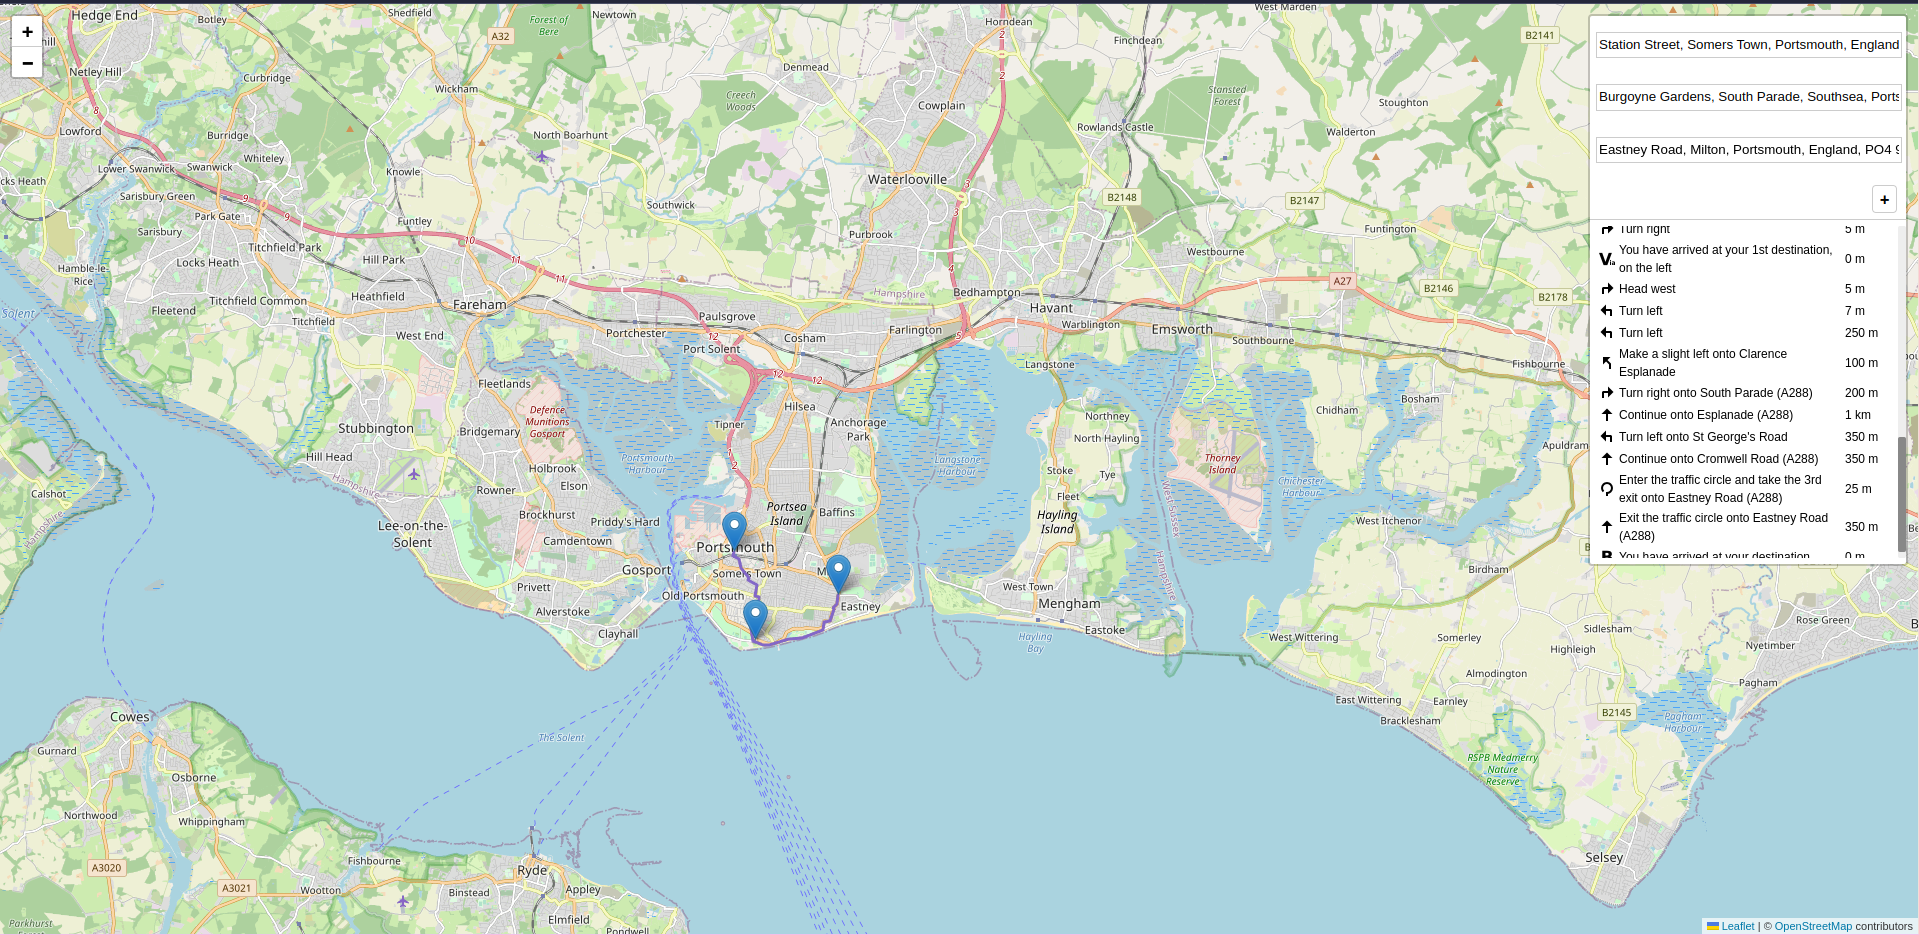
\includegraphics[width=425px]{figures/Progress Images/Iteration-1/SR1/Basic Destination Overlay Set up.png}
    \caption{Routing UI}
    \label{fig:routing-ui}
  \end{figure}

\subsection{Elevation Chart}
\label{iteration1:elevation-chart}
To create an elevation chart, the component was declared, with the plan to use Chart.js (\cite{noauthor_chartjs_nodate}) to draw the plot on a canvas element. A div was created to hold the chart component, where the elevation data was gathered from a state variable called 'coordinates' which contained the route latitude, longitude points and the altitude/elevations for each point \see{fig:waypoint-arr}. The distance along the route for each elevation point is calculated by dividing the total route distance (taken from a state variable called 'summary') by the length of the 'coordinates' array. To ensure continuity between the map and the elevation plot, a simple feature was added to allow the user to hover over the elevation plot, with the matching point along the route being highlighted. This required the hover point on the chart's canvas element to be found, matching the hover value to the latitude and longitude with the respective point and drawing a circle element on the Leaflet map \see{fig:elevation-hover}.

\begin{figure}[!ht]
    \centering
    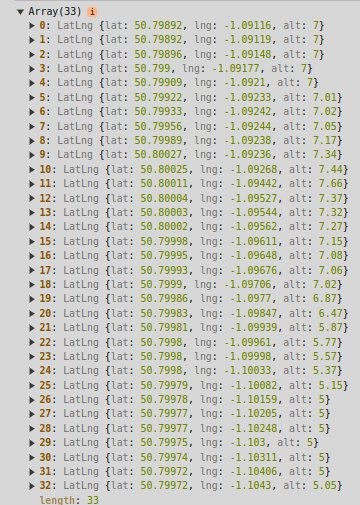
\includegraphics[width=200px]{figures/Progress Images/Iteration-1/SR1/waypoint-arr.png}
    \caption{Route Waypoint/Elevation Array}
    \label{fig:waypoint-arr}
  \end{figure}

\begin{figure}[!ht]
    \centering
    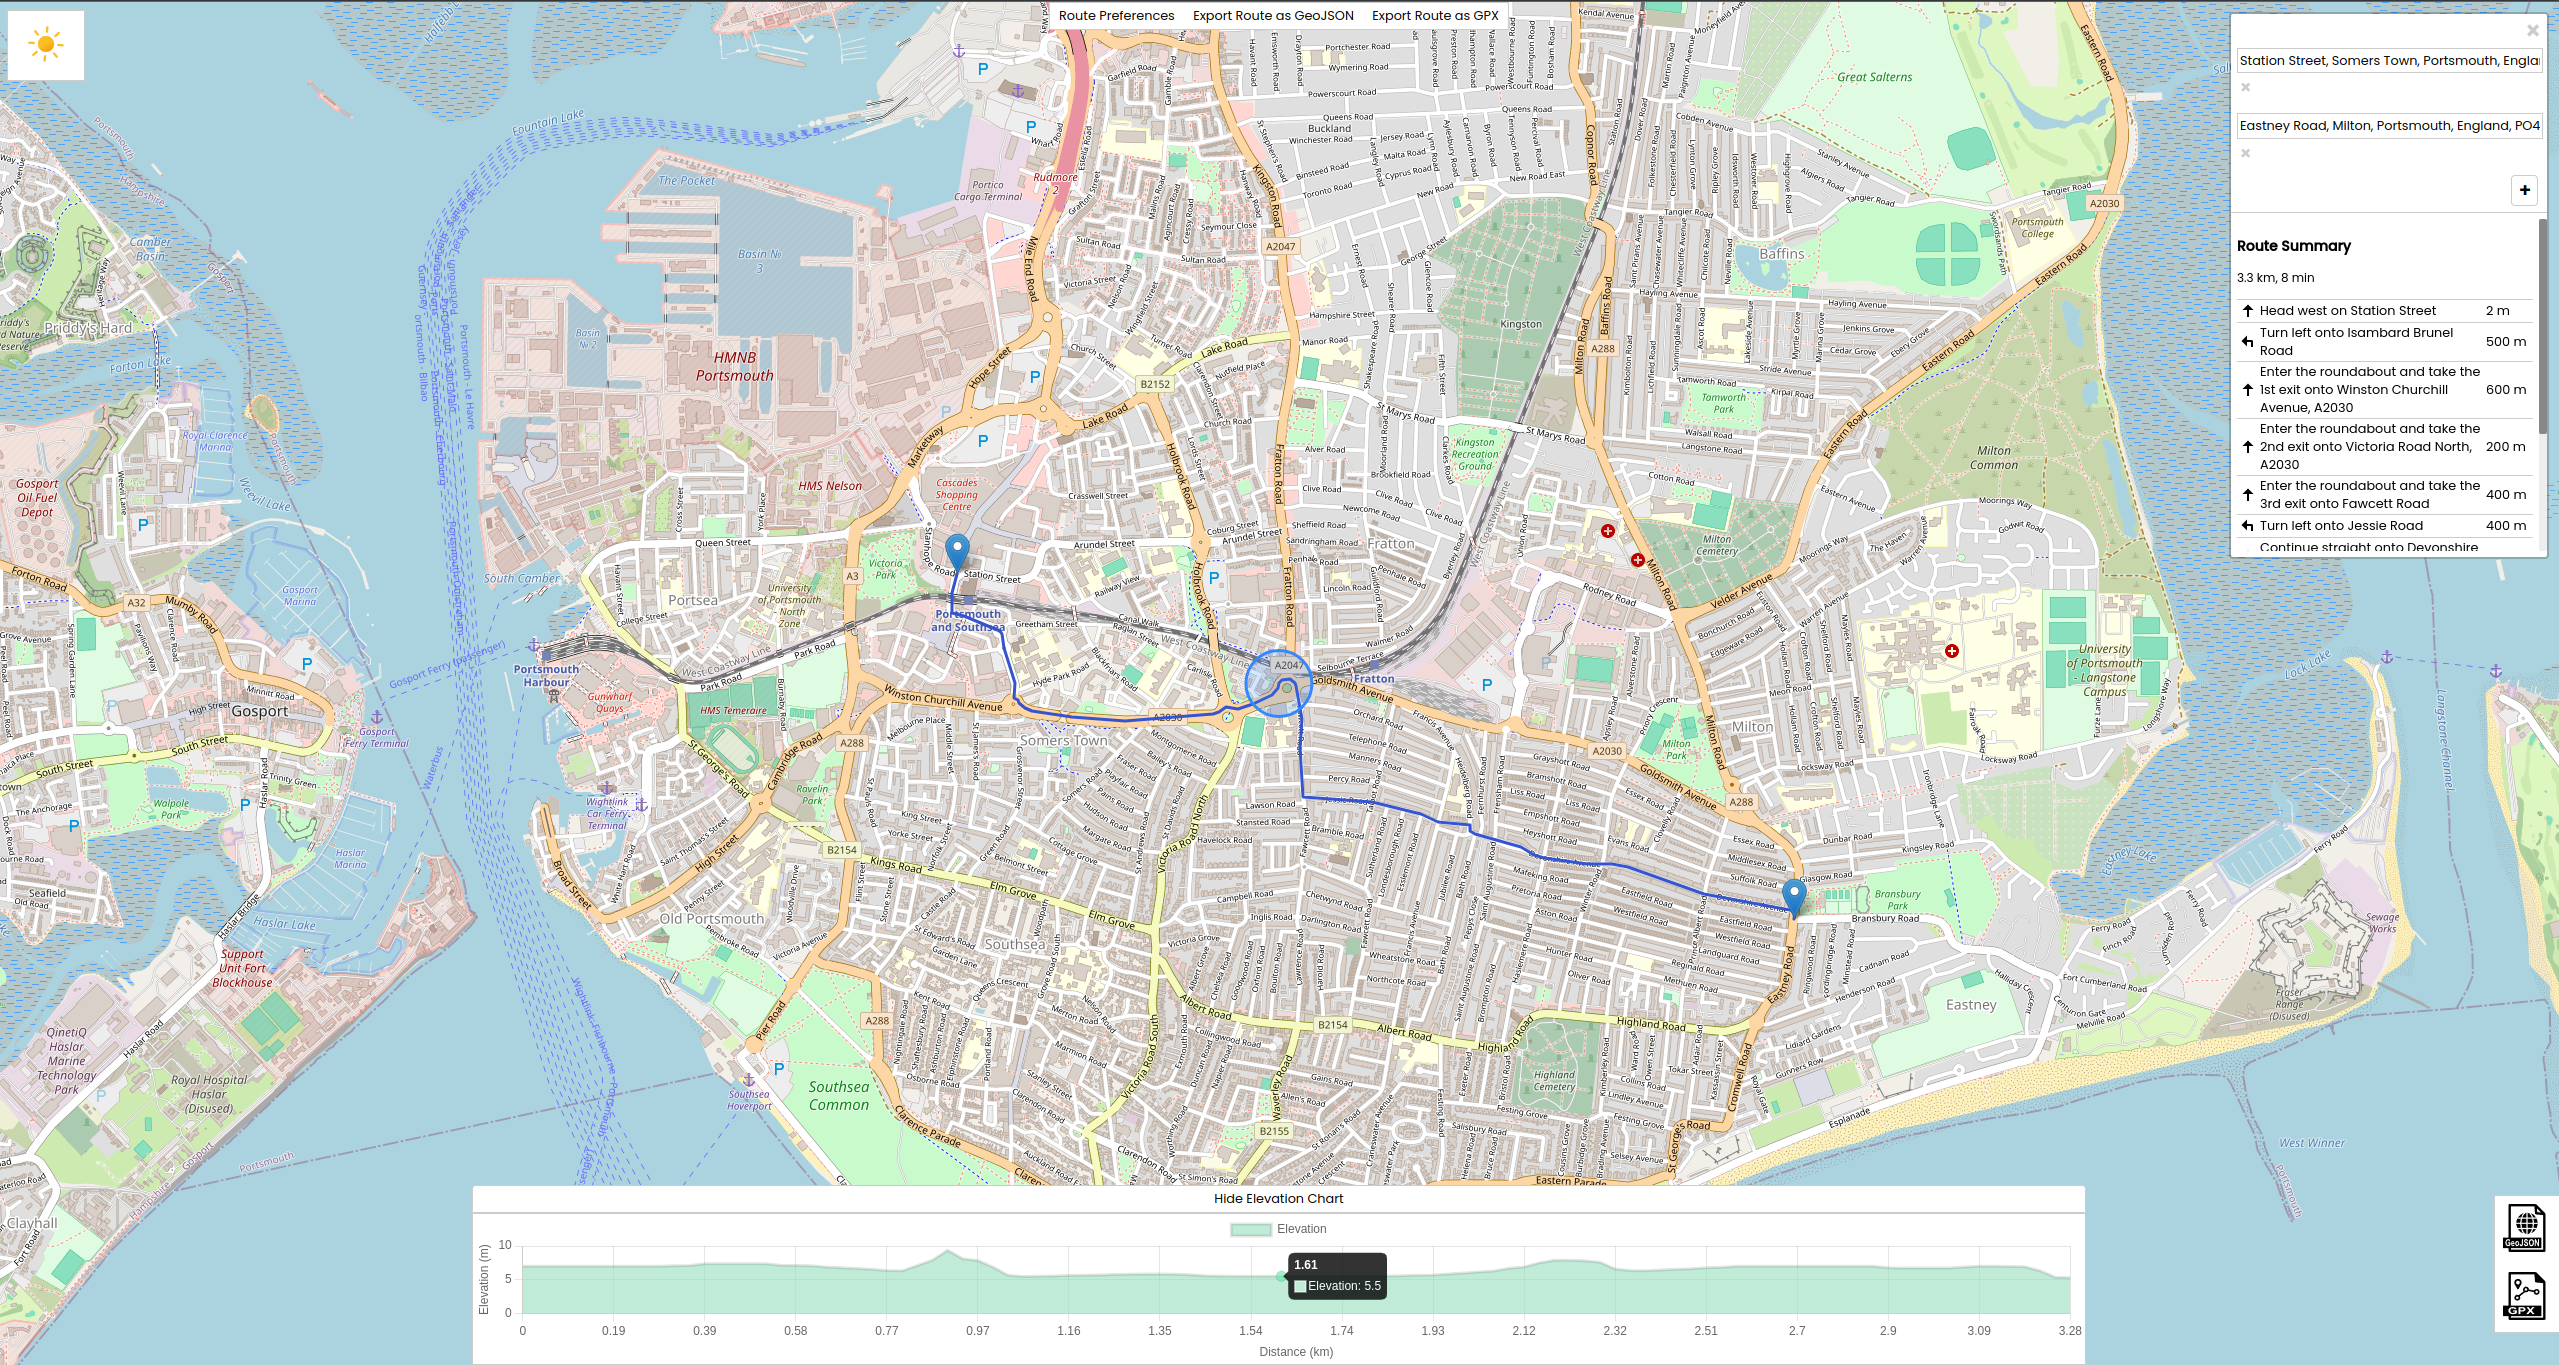
\includegraphics[width=425px]{figures/Progress Images/Iteration-1/SR28/elevation-hover.png}
    \caption{Elevation Plot Hover Functionality}
    \label{fig:elevation-hover}
\end{figure}

\subsection{Weather Information Panel}
\label{iteration1:weather-panel}
A generic weather panel was created within iteration 1, displaying weather information for the current day at the user's current location. The weather panel used the browser's geolocation API called within a React useEffect to get the user's general location, asking for permission via a pop-up window, then storing the geolocation in a state variable. The approximate coordinates returned from the API were then passed to Open Weather Map to gather all weather data for the current day. The Meteocons icons (\cite{noauthor_weather_nodate}) were used to display images demonstrating the current weather conditions \see{fig:basic-weather-panel}. The visibility of the weather panel was determined by a State variable, if the variable was true, the height and width of the panel expand, and when false, reduce to the button size.

\begin{figure}[!ht]
    \centering
    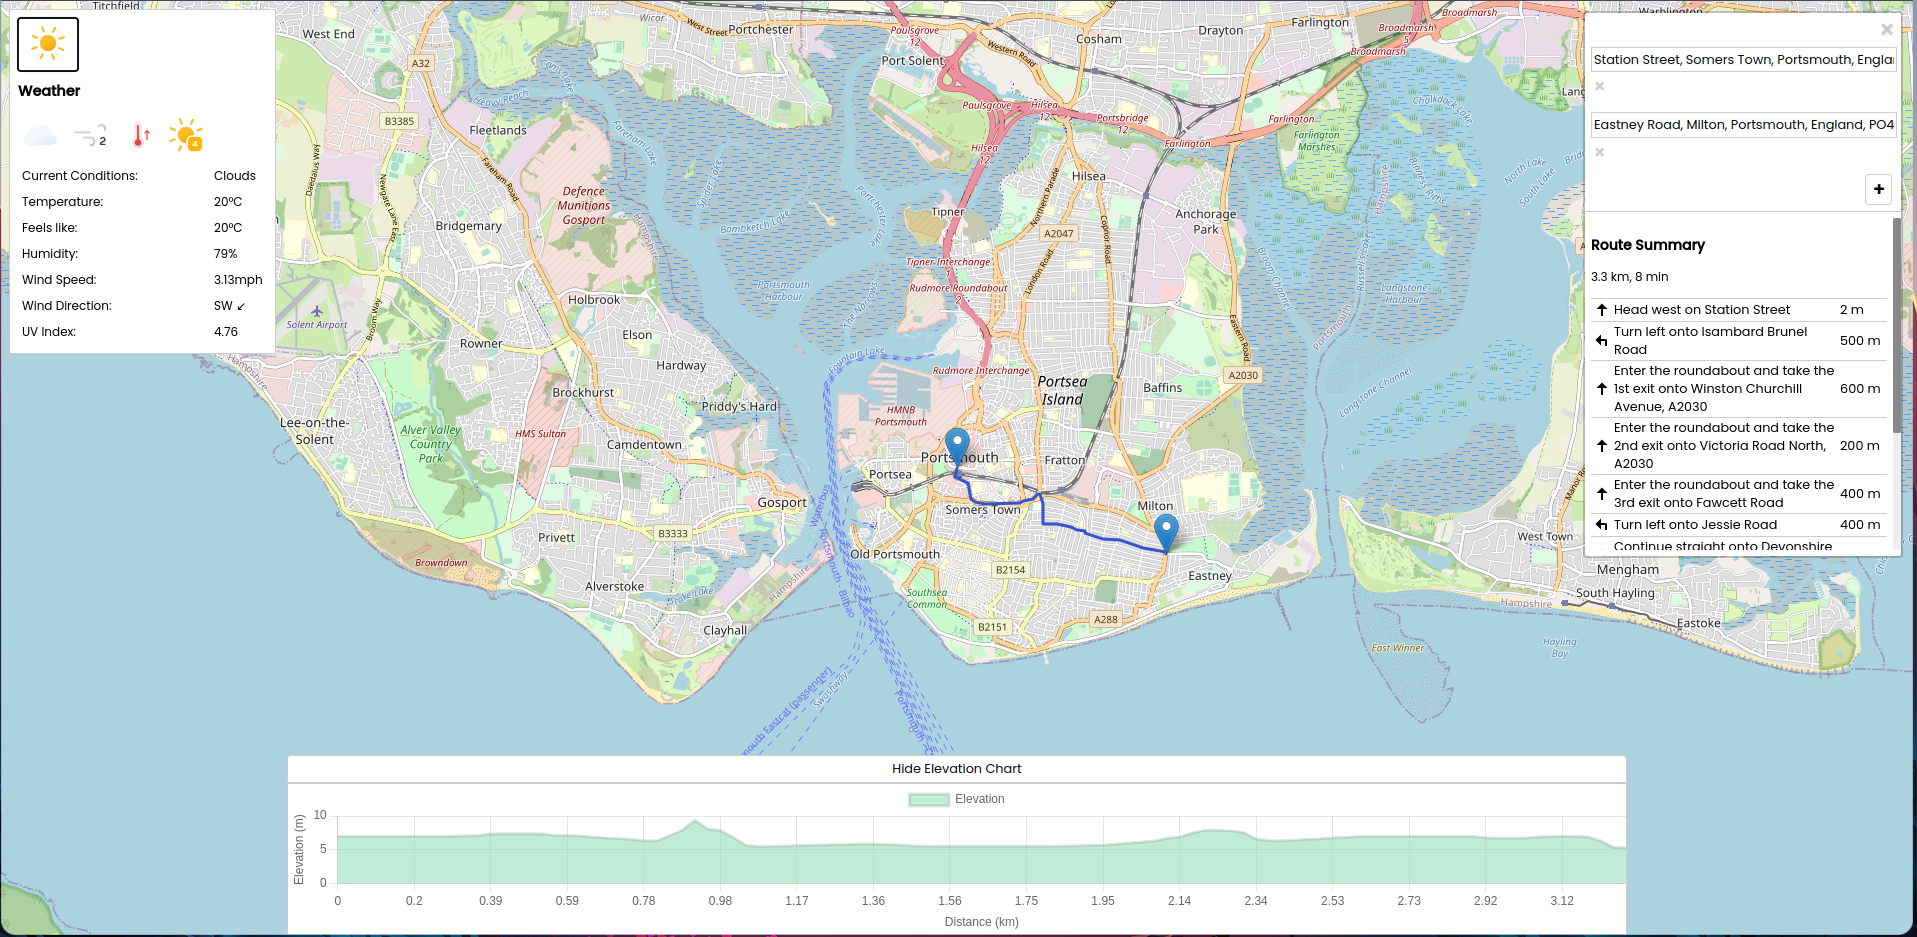
\includegraphics[width=300px]{figures/Progress Images/Iteration-1/SR19&SR28 Combined/SR19&SR28 Merged.png}
    \caption{Weather Panel}
    \label{fig:basic-weather-panel}
\end{figure}

\subsection{Main Challenges}
\label{iteration1:main-challenges}
The main challenge of Iteration 1 (i1), was primarily integrating multiple services to communicate seamlessly through the React.js frontend. Syncing hovering over the elevation plot, with a matching point along the route polyline, proved difficult. Despite the calculations being simple to determine at what latitude and longitude to draw the circle marker on the map when hovering on the plot, getting the map instance reference was more difficult than expected. Initially, the reference would return undefined, therefore no marker was drawn on the map, however after implementing a useState and declaring a local copy of the map instance, the hover functionality worked seamlessly.

Furthermore, the only other challenge faced was retrieving the user's geolocation from the browser. A useEffect was required to access the geolocation API, however, the useState was at first missed to store the geolocation value once the API had returned the data. Once the state variable was added, however, the weather panel would re-render once the data was retrieved.

\section{Iteration 2 - Route Sharing, Hazard Index and POI Integration}
\label{implementation:iteration2}

Unlike i1, Iteration 2 (i2) development was conducted after the primary research and requirements review had been completed. The remaining updated requirements were prioritised and distributed between i2 and Iteration 3 (i3) \see{implementation:iteration3}. I2 builds on i1, enhancing existing functionality and introducing new features throughout the iteration. 

\subsection{Sharing Route Functionality}
\label{iteration2:sharing-route}

Route sharing was implemented with i2, when routes were found using Open Route Service, GPX (\cite{noauthor_gpx_nodate}) and GeoJSON (\cite{noauthor_geojson_nodate}) strings were generated. These files were then used to create a share to email feature using the Twilio SENDGRID API (\cite{noauthor_email_nodate}). Initially, it was planned to send emails direct to the SENDGRID directly from the client, to mitigate the middle-man required to send the request, however it was found that SENDGRID would only accept incoming requests from the server. Therefore, an API endpoint was created with Gin to handle the POST request from the frontend. 

Each email would contain a simple amount of predefined text with the included GPX and/or GeoJSON files selected for export. A modal was created to display the email form, where the user could input the recipient's email address, route name and choose what type of file to share \see{fig:basic-weather-panel}.

Initially, it was planned to use the Strava API to upload GPX files directly to the user's Strava Routes account, however, it was found that the Strava API had no such endpoint to integrate with routes. It was decided to still implement Strava integration, but with activities, enabling route export as an activity for users without dedicated fitness devices. 

A modal was created \see{fig:strava-modal} and a POST request endpoint set up to handle the request to the Strava API. The user would be required to log in to their Strava account, to enable the artefact access to upload activities. Once logged in, the user could select the route to upload, then the artefact would send the GPX file to the Strava API, where it would be converted to an activity and stored in the user's account \see{fig:strava-example}.

\begin{figure}[!ht]
  \centering
  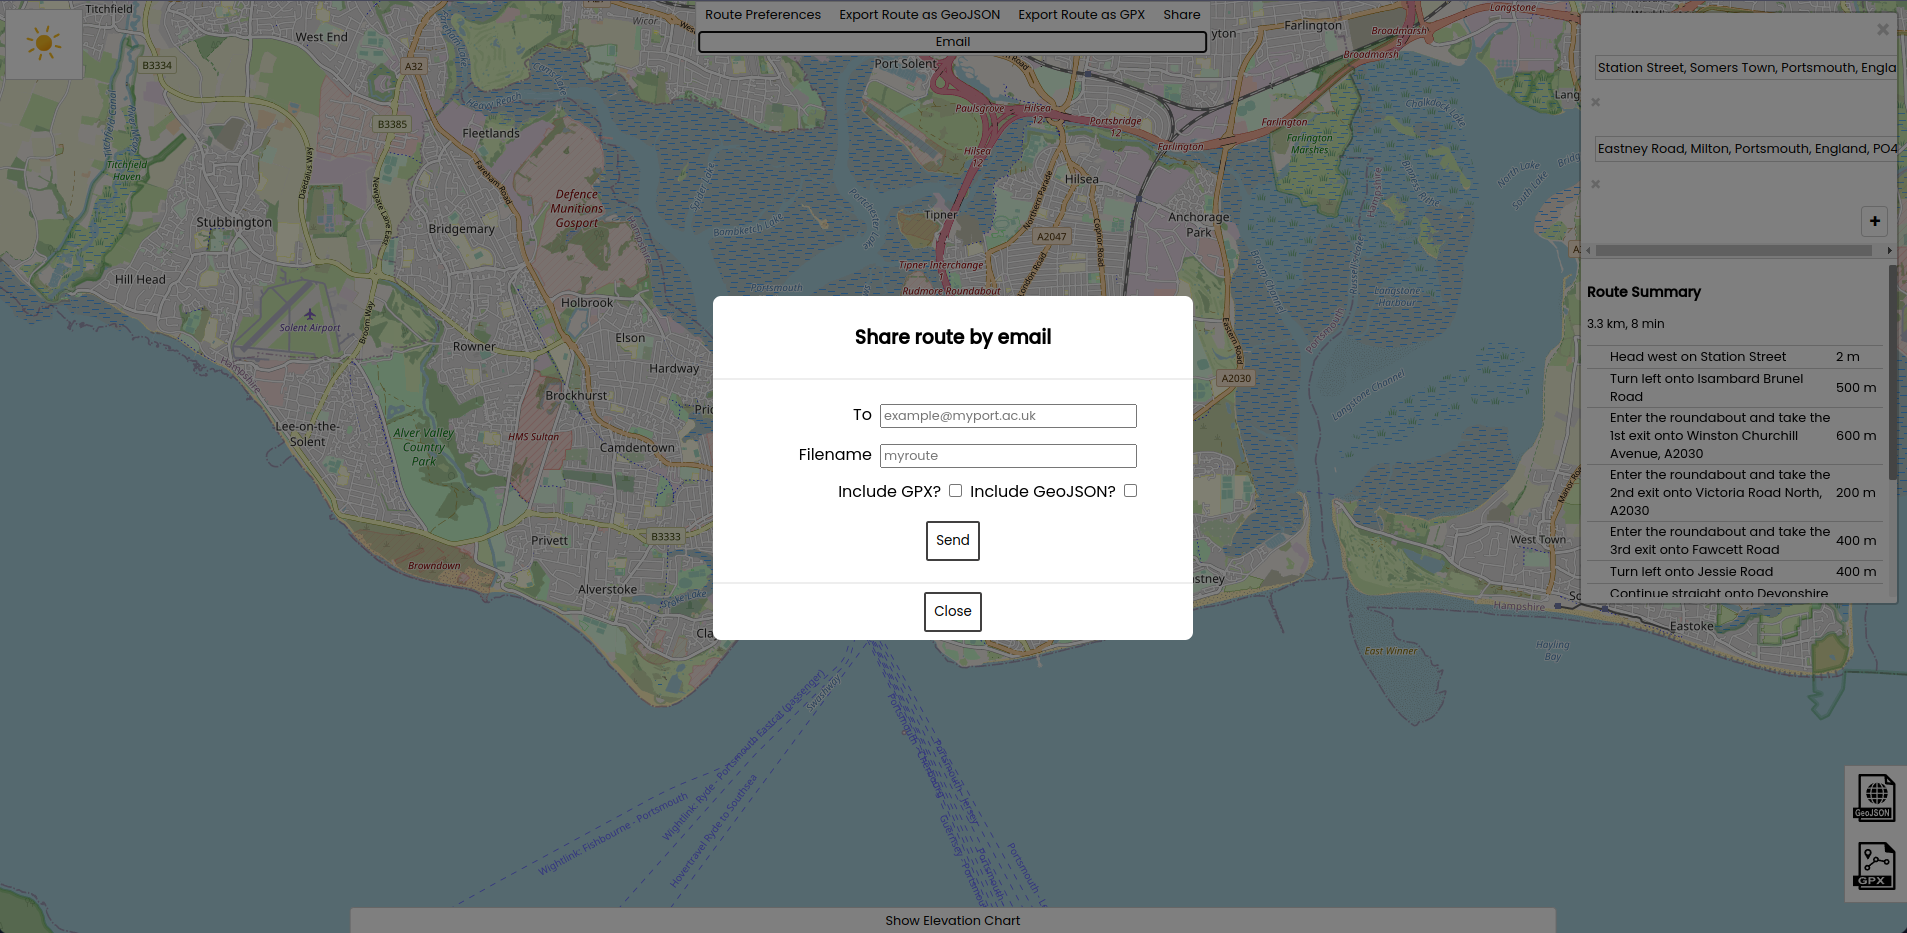
\includegraphics[width=425px]{figures/Progress Images/Iteration-2/SR17/SR17png.png}
  \caption{Share to Email Modal}
  \label{fig:share-email-modal}
\end{figure}

\begin{figure}[!ht]
  \centering
  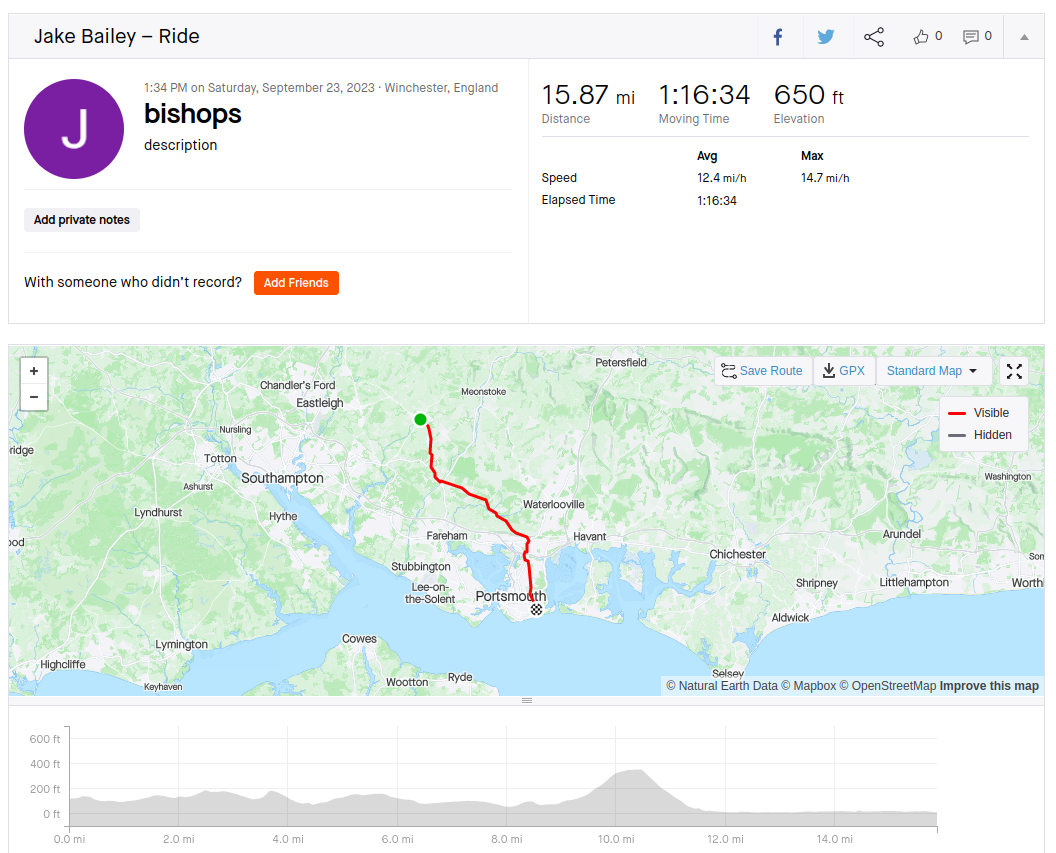
\includegraphics[width=425px]{figures/Progress Images/Iteration-2/SR18/SR18 Upload Example 1.png}
  \caption{Strava Activity}
  \label{fig:strava-example}
\end{figure}

\begin{figure}[!ht]
  \centering
  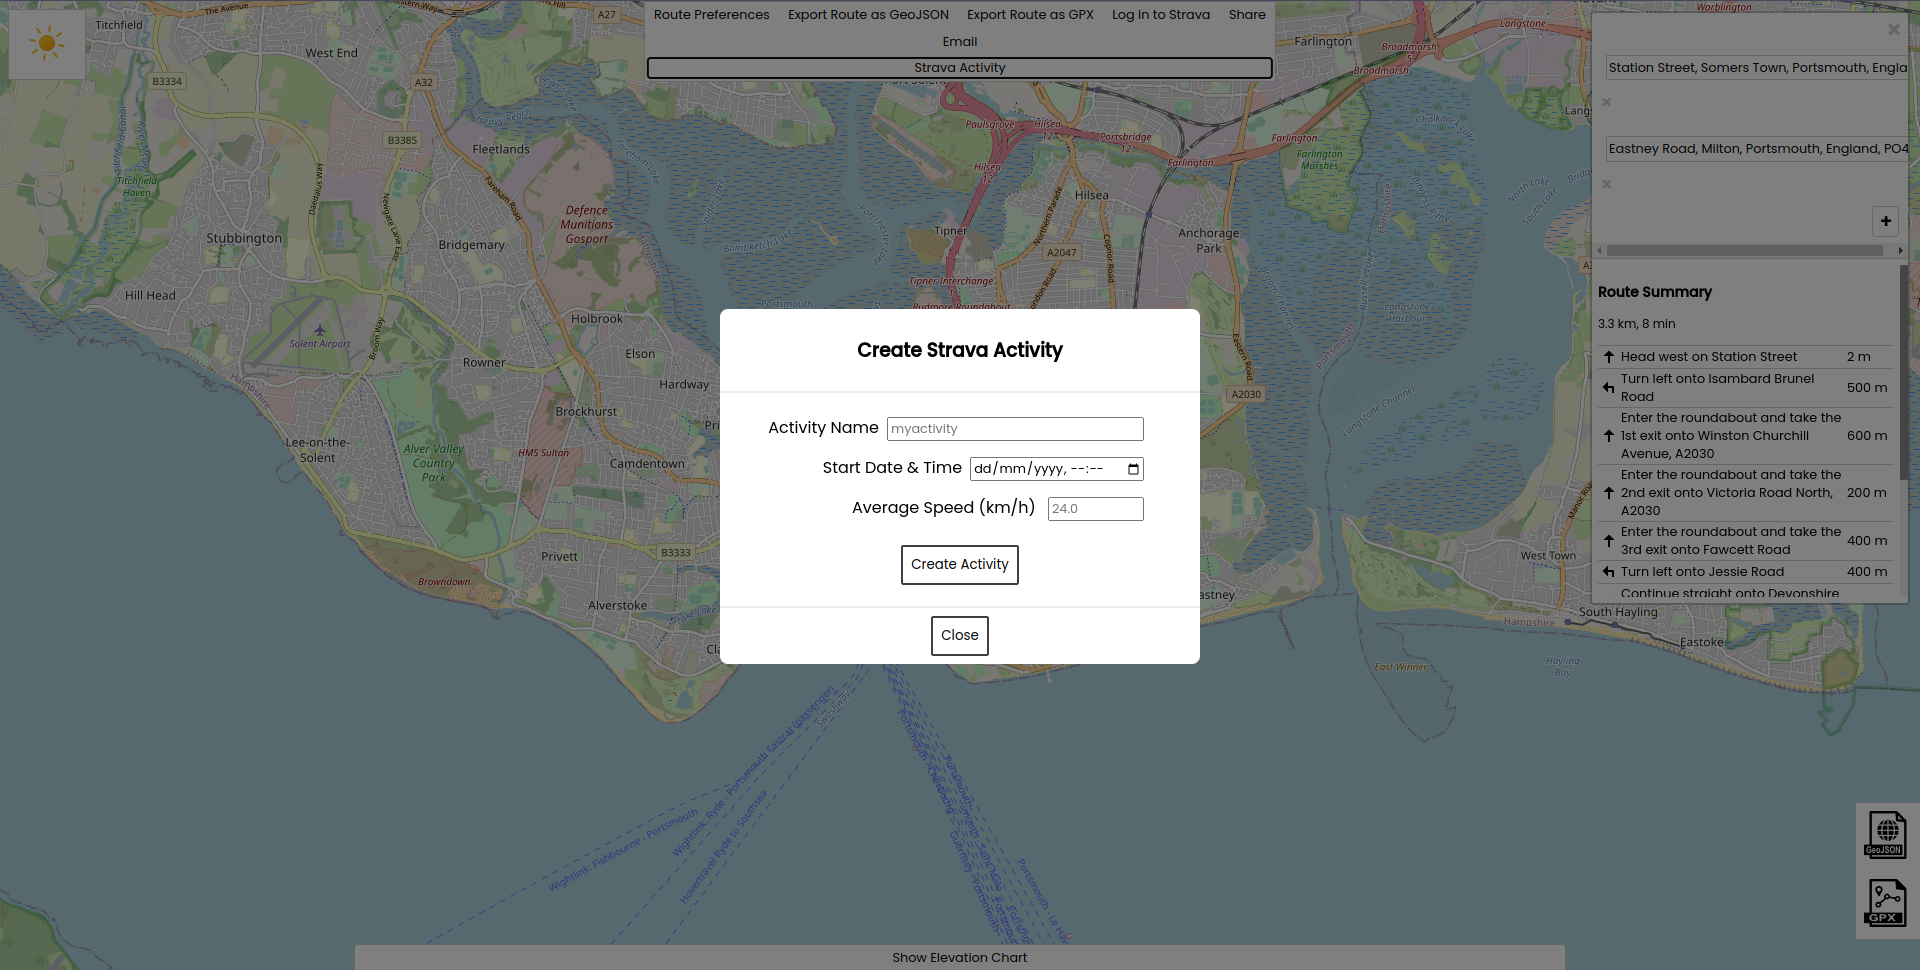
\includegraphics[width=425px]{figures/Progress Images/Iteration-2/SR18/SR18 Strava Modal.png}
  \caption{Share to Strava Modal}
  \label{fig:strava-modal}
\end{figure}


\subsection{Hazard Index Database Creation and Integration}
\label{iteration2:hazard-index}

Creation and integration of the hazard index database was the largest task of i2. The database was created using PostgreSQL using PostGIS. The database was split into eight tables representing a hazard, related details and its geospatial data \see{system:database-design}. Hazard types were chosen based on the most relevant hazards defined on the Open Street Map wiki (\cite{noauthor_keyhazard_nodate}) with the addition of a 'Cycling Infrastructure' hazard. The 'Cycling Infrastructure' hazard type was added to allow users to report and view bad cycling infrastructure in their area, with the intention of routing algorithms avoiding these areas in the future.

To integrate the database into the artefact, API endpoints were created to handle GET and POST requests to the database. The database was connected to the Go backend using the 'github.com/lib/pq' package (\cite{noauthor_pq_nodate}), with Gin handling the routing of requests to the database. Using the fetch API, the frontend could make API calls, to add and retrieve hazards from the database, supplying coordinates for the hazard location/area and the hazard type \see{fig:hazard-creation}.

To enable users to contribute to the hazard index database, a UI was created using the Leaflet Draw API (\cite{noauthor_leaflet_nodate-2}). The API allowed a few controls to be added to the map, including buttons to draw markers and polygons onto the map. These buttons were used to create a hazard, where I implemented an event handler to catch the polygon/marker drawn once completed. This event handler would then proceed to make open the hazard creation modal, with the coordinates of the drawn polygon/marker passed to the modal via props. The user could then add the extra information required for the hazard and submit the hazard to the database.

Furthermore, to display the hazard data on the map, a new layer must be created. The layer was added to the map using the React Leaflet library, where the hazards were retrieved from the database and drawn on the map. These hazards were shown as both markers and polygons to represent a point or area hazard \see{fig:hazard-layer}. The API endpoint was set up to allow the user to retrieve all hazards within a five mile radius of a point, to enable the user to see hazards in their area, as the map was panned, the hazard layer would update \see{fig:hazard-API}.

\begin{figure}[!ht]
  \centering
  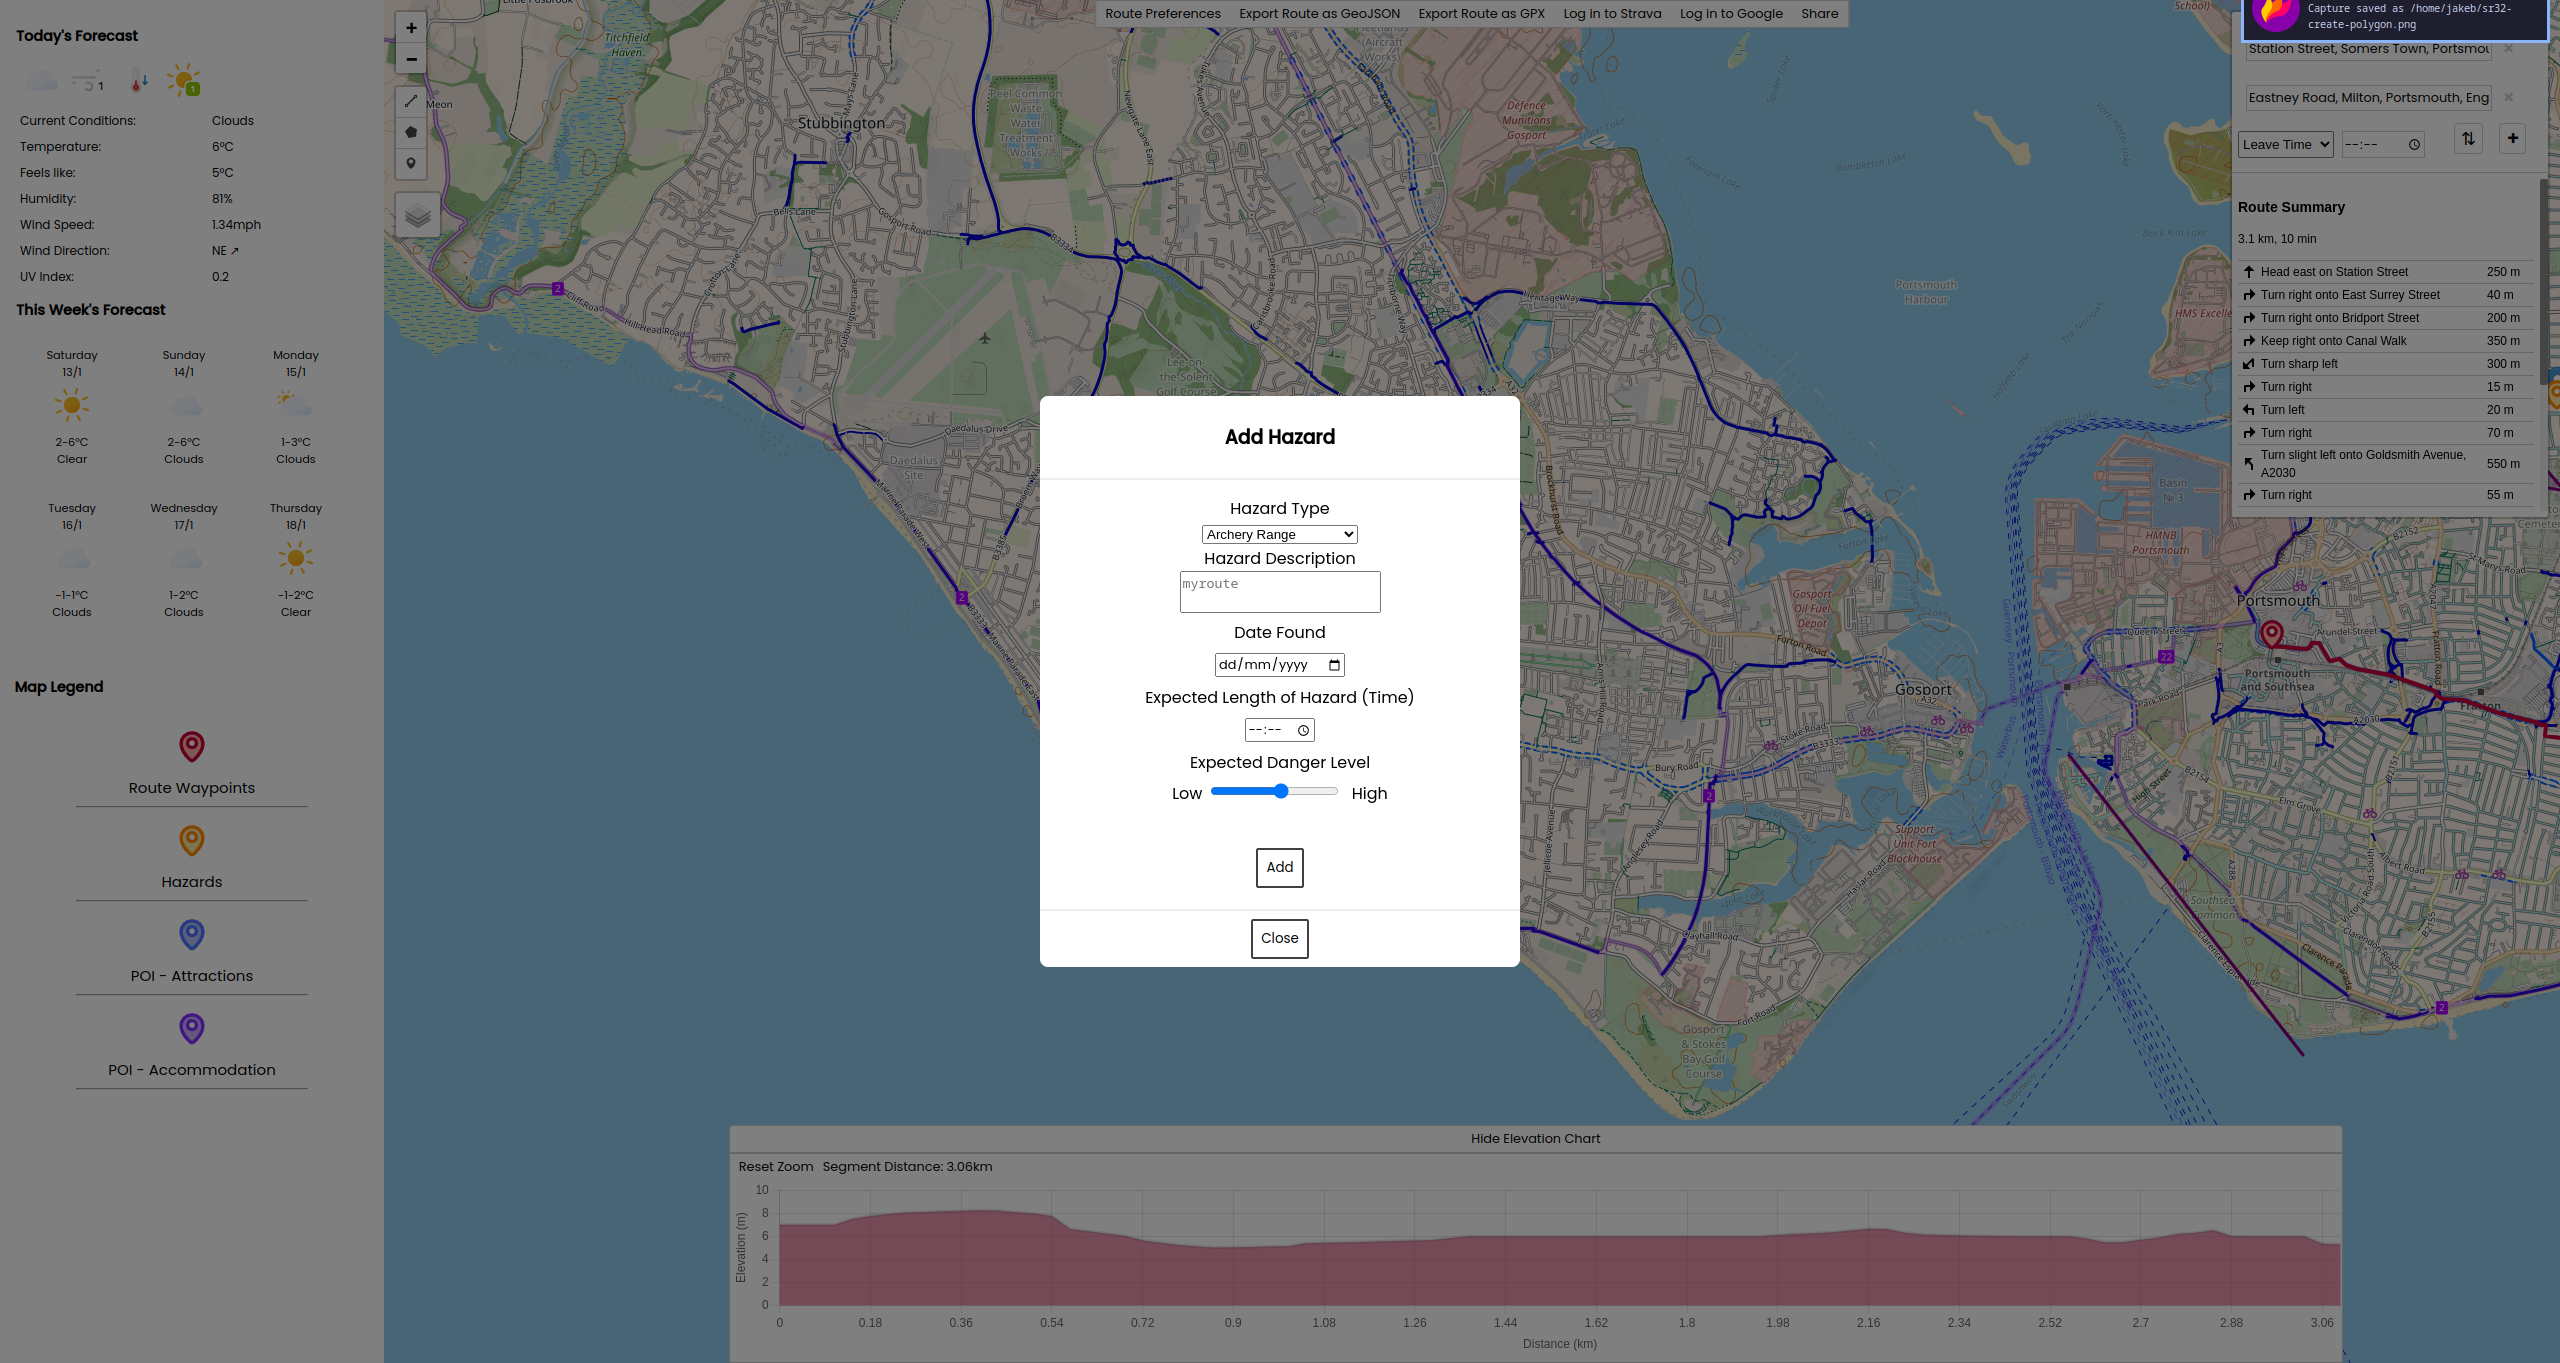
\includegraphics[width=425px]{figures/Progress Images/Iteration-2/SR32-37/sr32-add-hazard-point.png}
  \caption{Hazard Creation Modal}
  \label{fig:hazard-creation}
\end{figure}

\begin{figure}[!ht]
  \centering
  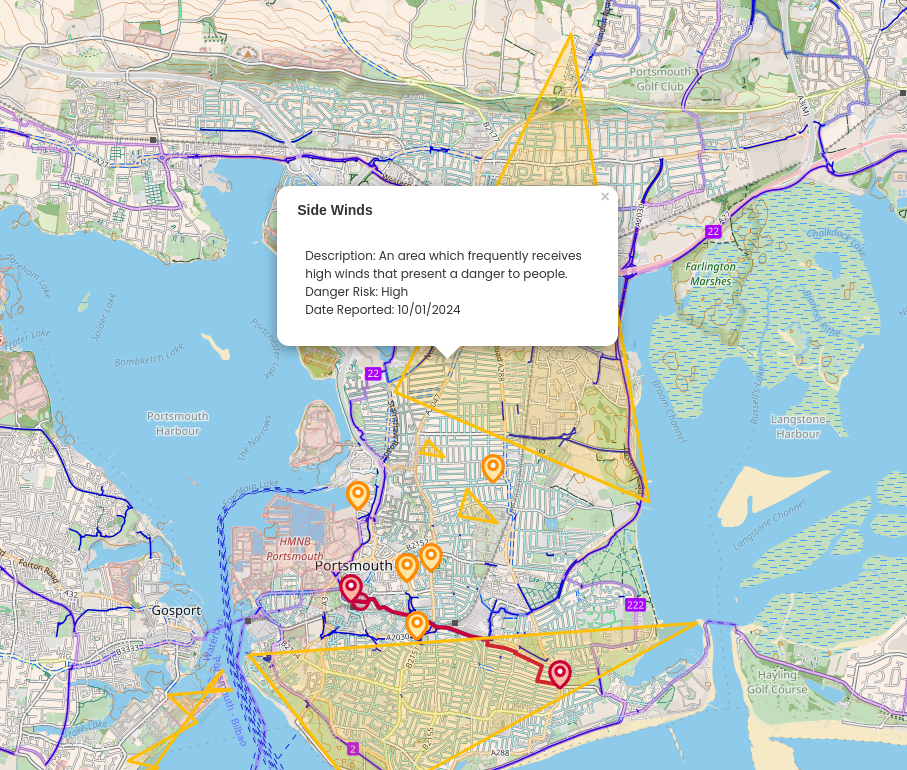
\includegraphics[width=300px]{figures/Progress Images/Iteration-2/SR32-37/sr32-hazard-popup.png}
  \caption{Hazard Map Layer}
  \label{fig:hazard-layer}
\end{figure}

\begin{figure}[!ht]
  \centering
  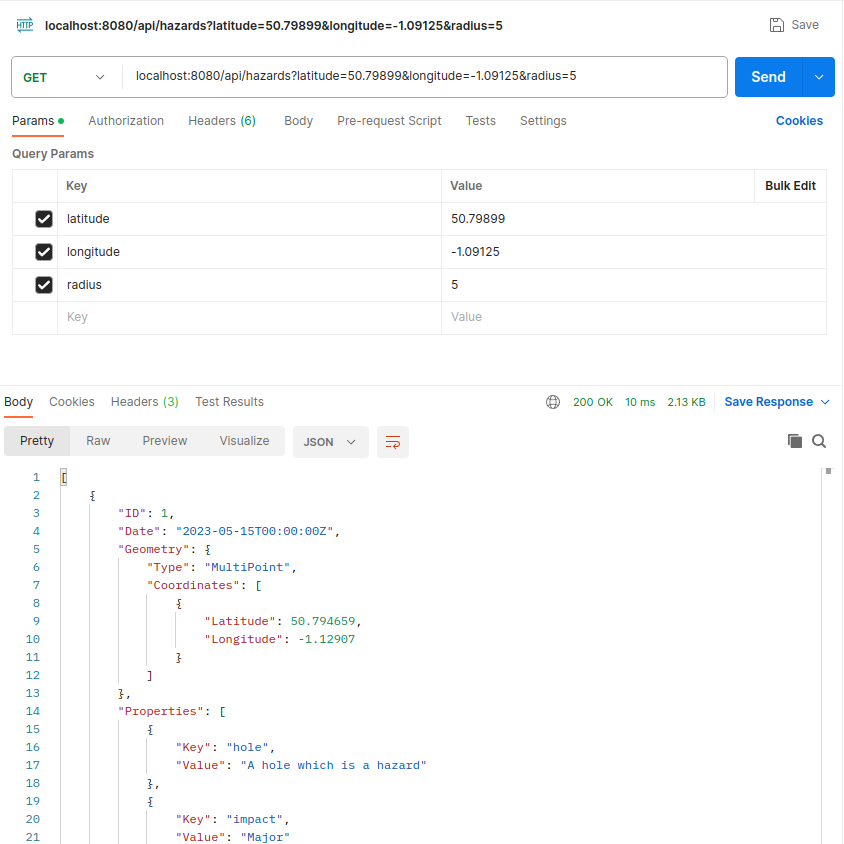
\includegraphics[width=425px]{figures/Progress Images/Iteration-2/SR32-37/SR32 - Basic API further developed.png}
  \caption{Hazard API Query}
  \label{fig:hazard-API}
\end{figure}

\subsection{Key Point-of-Interest (POI) Integration}
\label{iteration2:poi-integration}

The POI integration was the final feature of i2, where the user could view points of interest in their area. The POI data was retrieved from the Foursquare Places API (\cite{noauthor_places_nodate}). Two separate map layers were created similar to the hazard layer \see{iteration2:hazard-index}, one to display accommodation POI and another to display the attractions/leisure POI \see{fig:poi-layers}. The layer also allowed the user to click on each POI marker to view more information about the location, such as the name and address.

After the core POI layers were developed, two buttons were then added to each POI popup window. These were to allow a user to either route to or via the POI. If the user chose to route to, the last route waypoint would be updated to the POI's latitude and longitude. Whereas to route via, the route waypoints would initially be taken to find which route waypoint was closest to the POI, it would then be inserted into waypoints before the closest waypoint. The route would then be recalculated to include the POI as a waypoint \see{fig:poi-route}.

\begin{figure}[!ht]
  \centering
  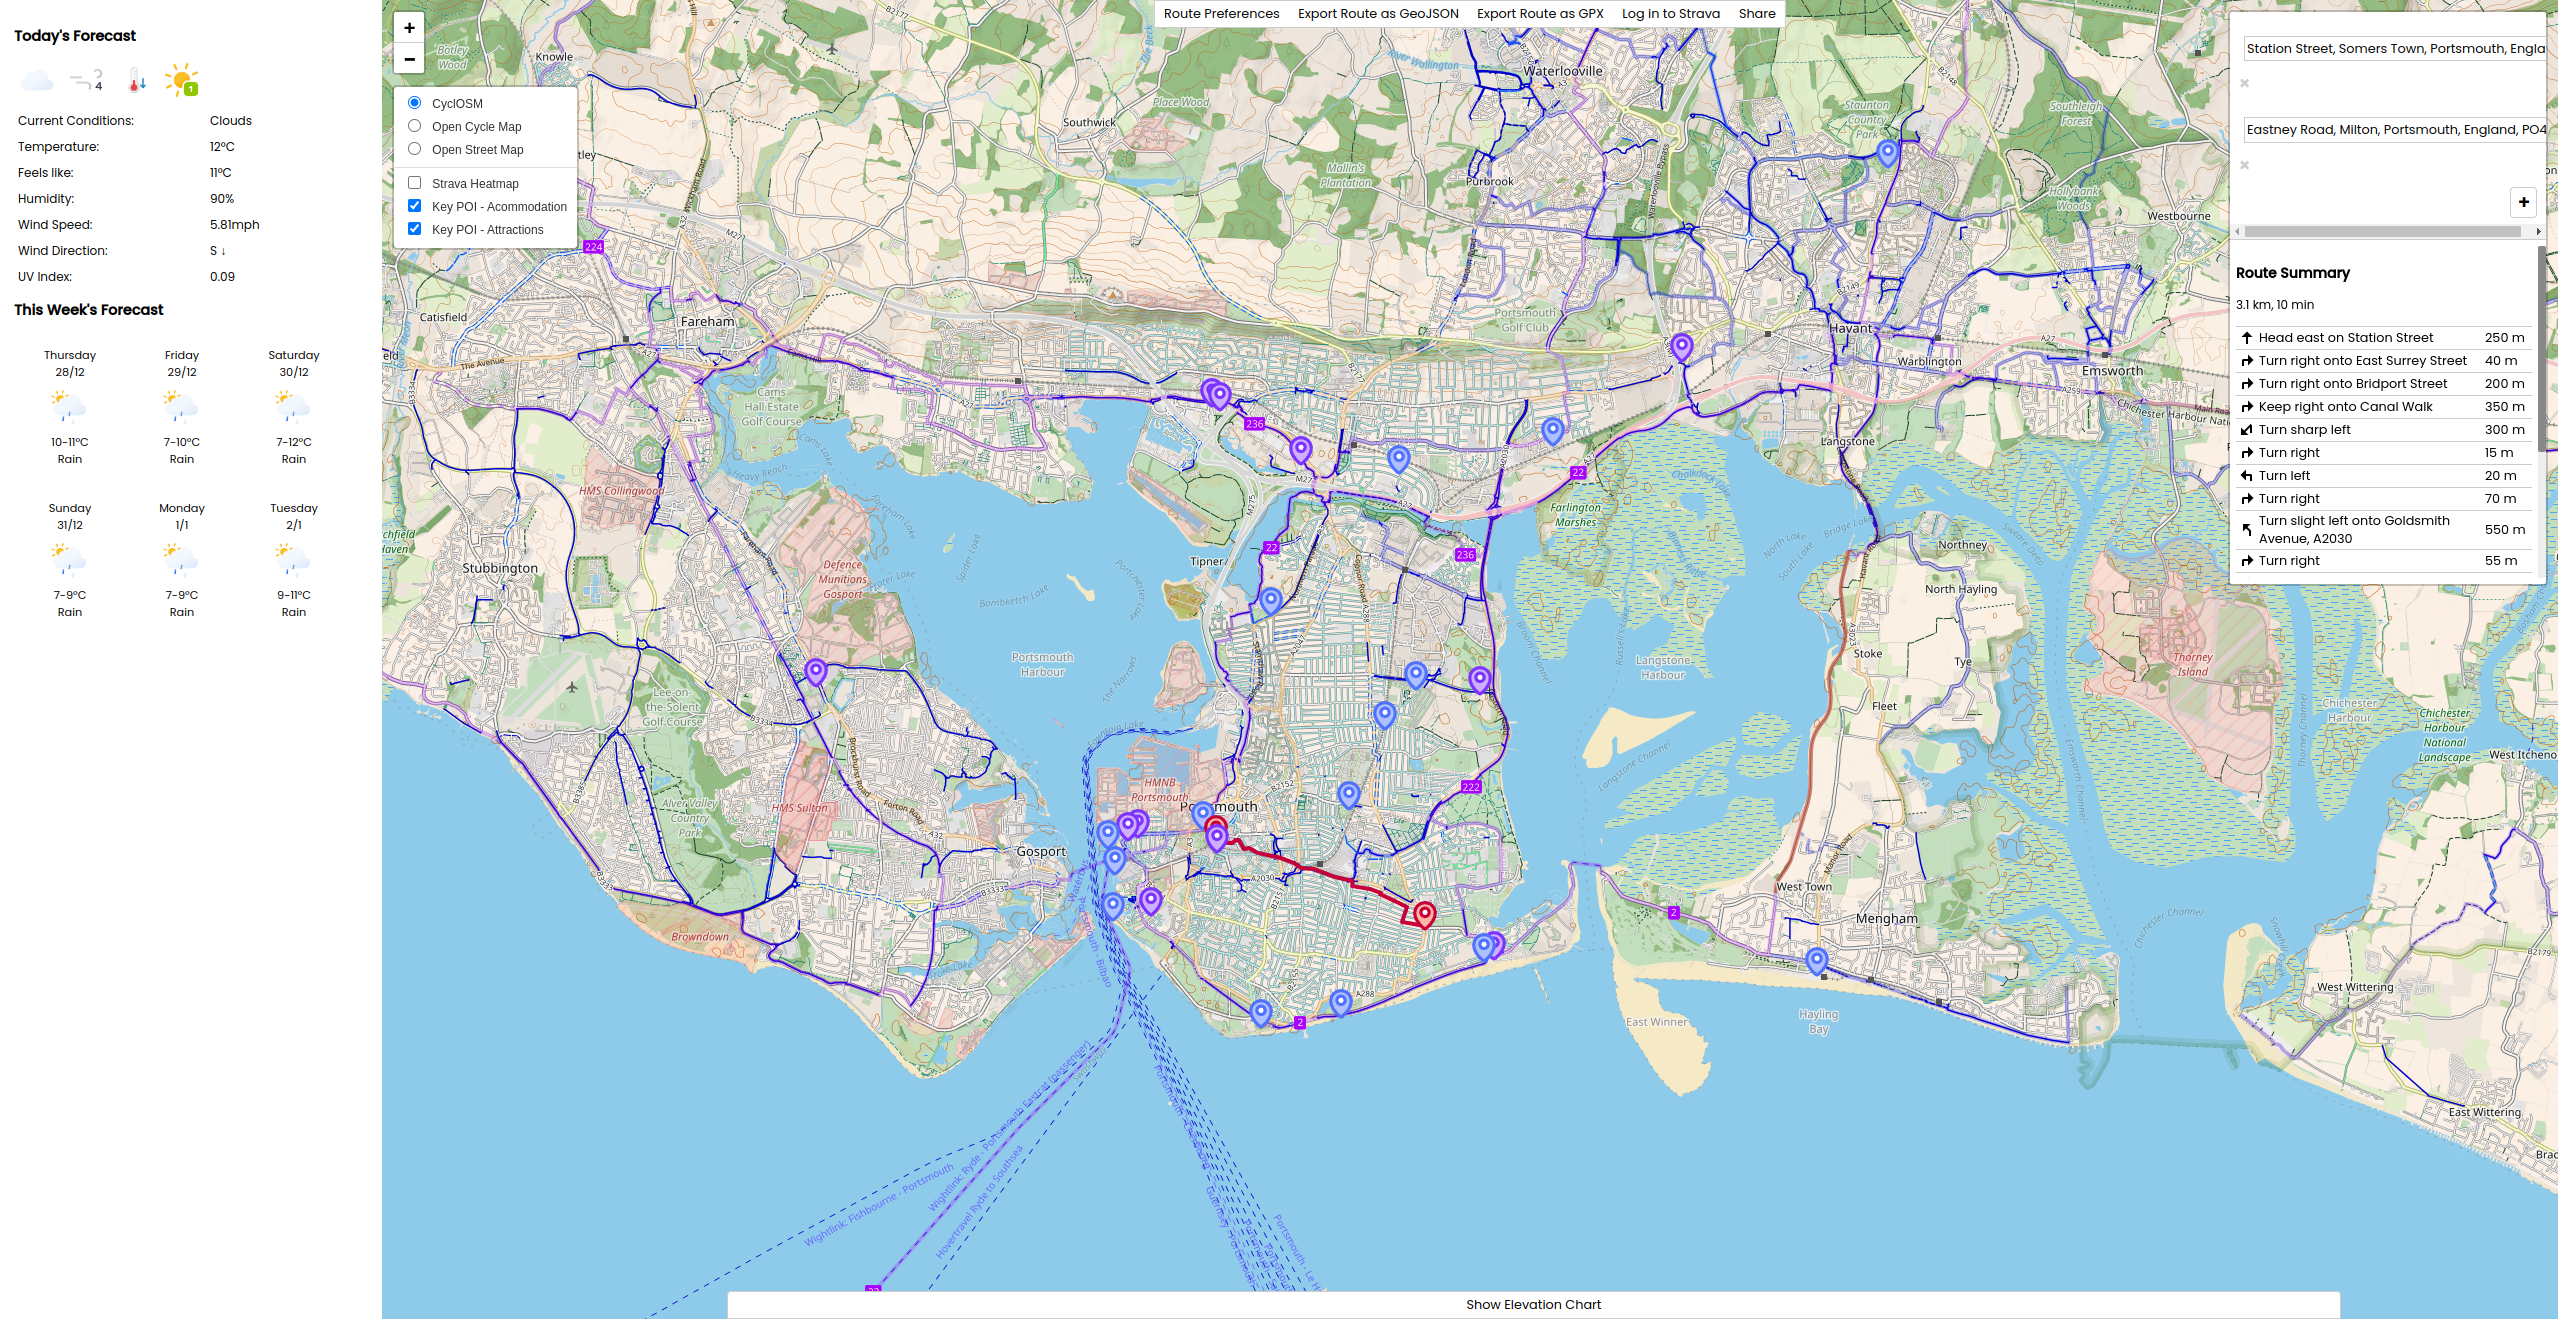
\includegraphics[width=425px]{figures/Progress Images/Iteration-2/SR40-45/SR40 - Attractions and Accommodation KeyPOI.png}
  \caption{Attractions and Accommodation Layers}
  \label{fig:poi-layers}
\end{figure}

\begin{figure}[!ht]
  \centering
  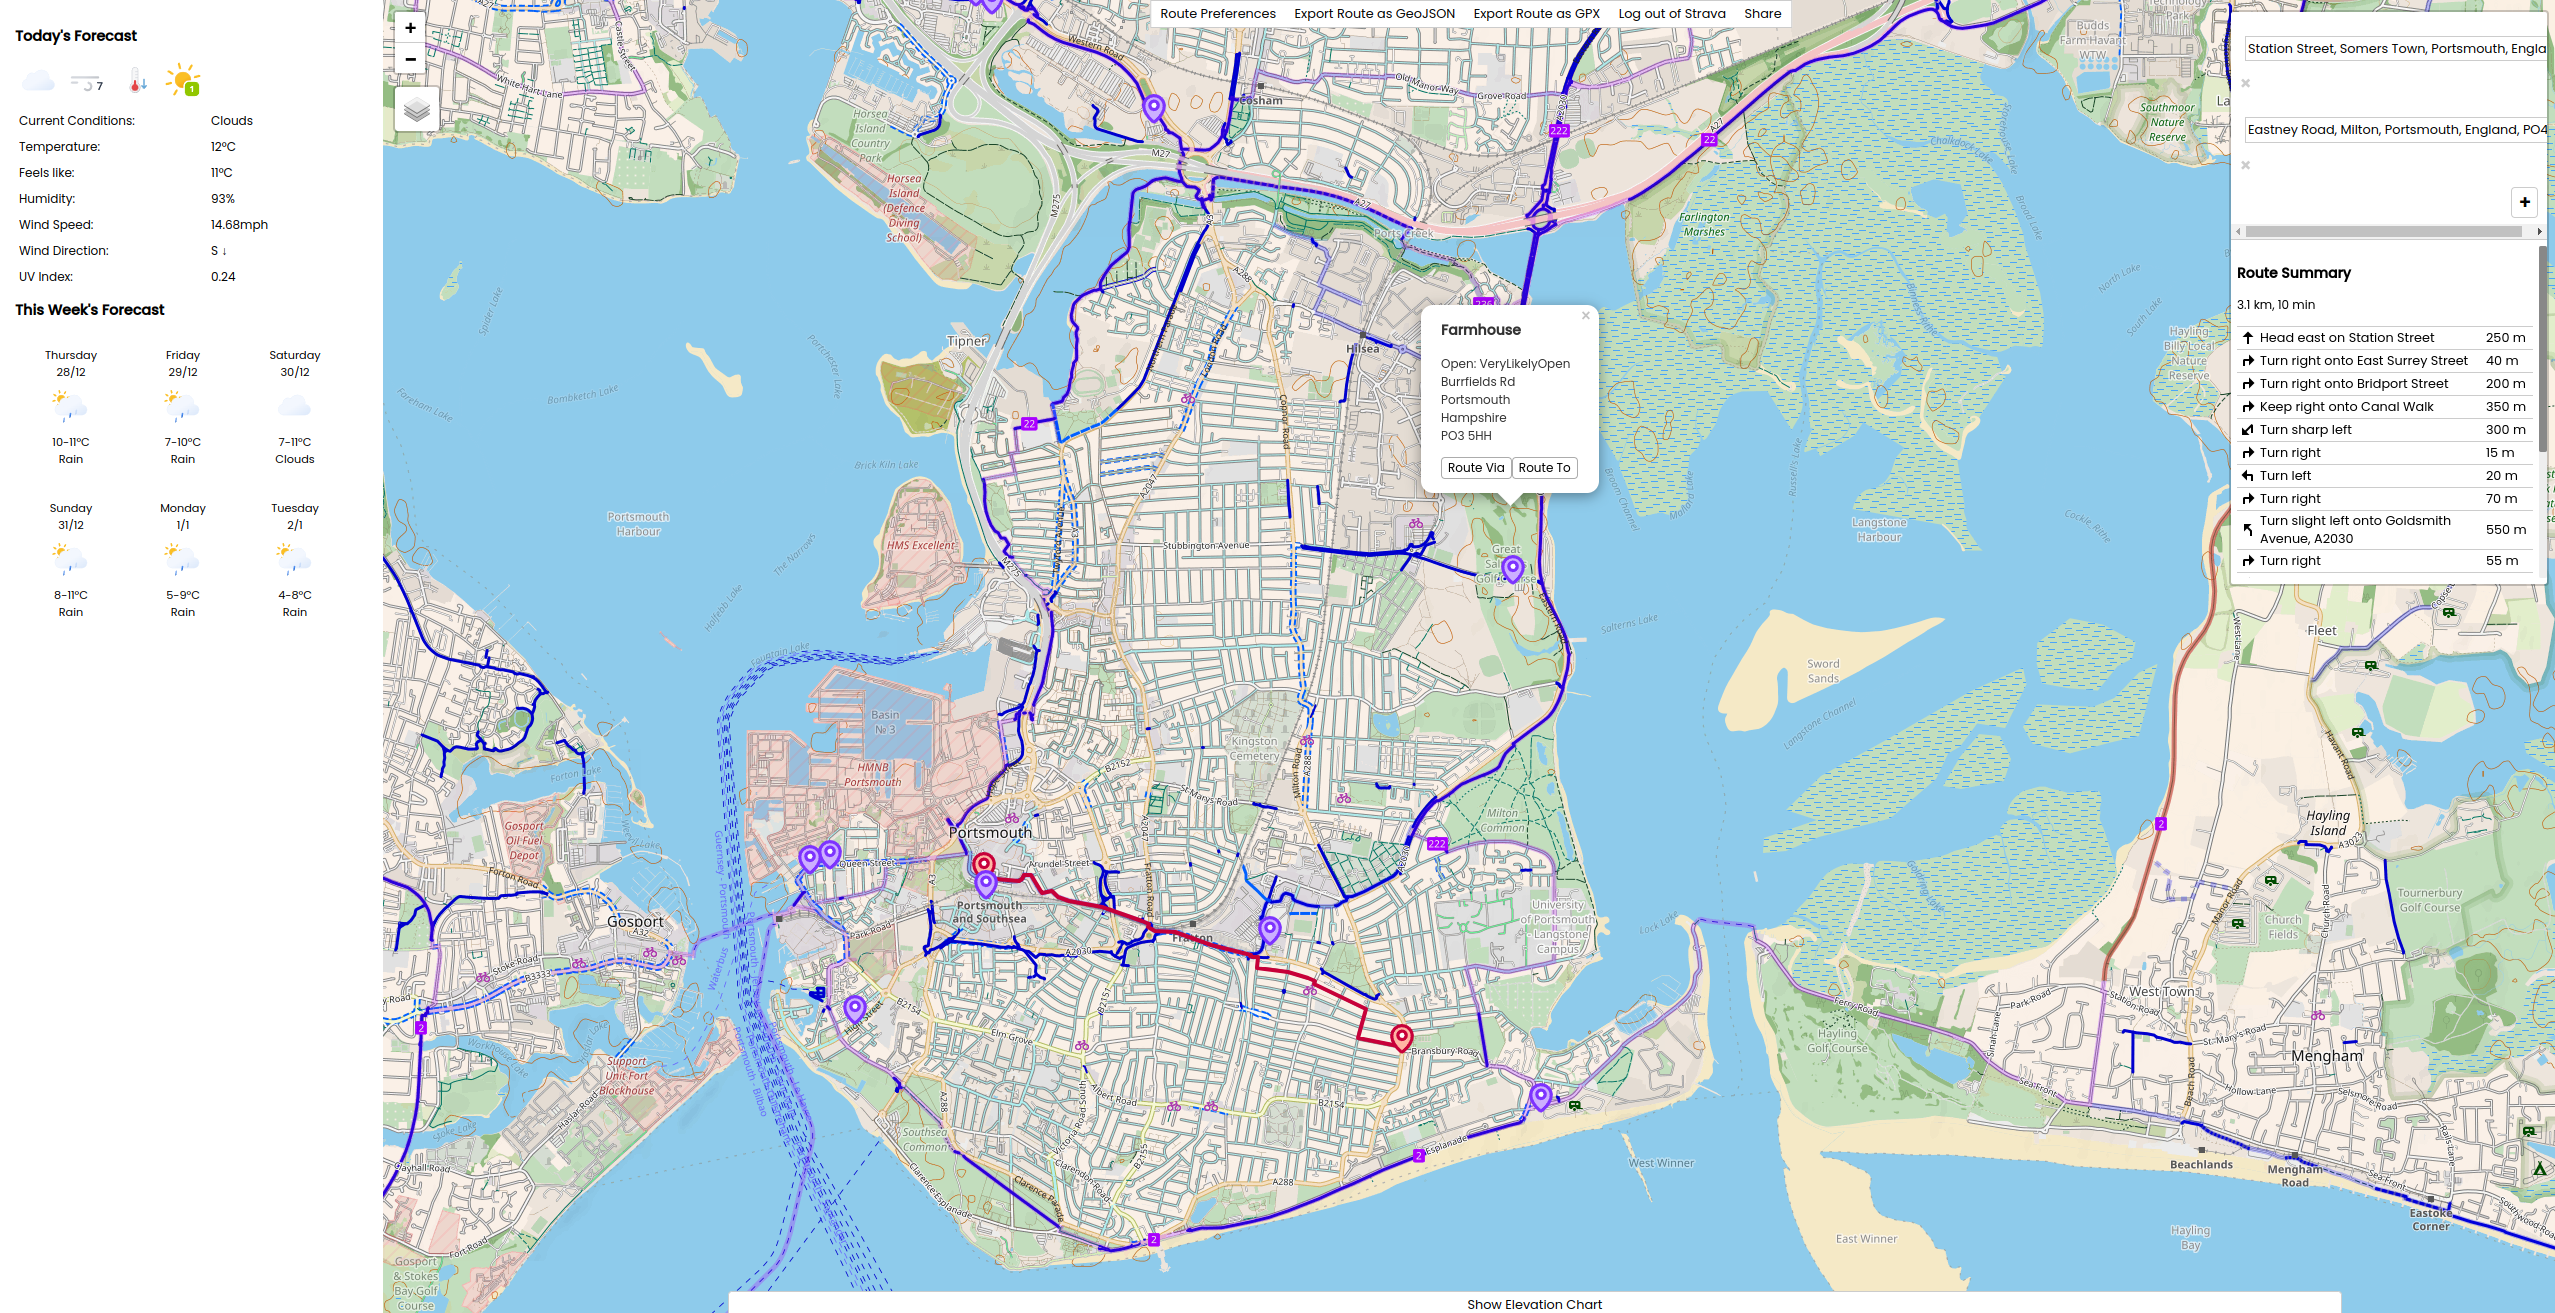
\includegraphics[width=425px]{figures/Progress Images/Iteration-2/SR40-45/SR45 - Route ToVia POI.png}
  \caption{Route To/Via POI}
  \label{fig:poi-route}
\end{figure}

\subsection{Main Challenges}
\label{iteration2:main-challenges}

The main challenges for i2 resided in setting up the SQL queries to handle the hazard data requests as well as oauth authentication with the Strava API.

The INSERT hazard query was the most complex. The PLpgSQL language was used to create a function to handle  this logic as loops were required when inserting multiple PostGIS Point data types (coordinates) for each hazard. A loop was also required to insert the properties for each hazard, where each hazard could have one or more. The function was then called from the API endpoint, passing the json string input directly into the PLpgSQL function as type JSONB.

The Strava API was also challenging as it was required to implement oAuth 2.0 manually to authorise the application to upload activities to the user's account. The Strava API documentation was relatively clear on how to implement this process, however, having not manually implemented oAuth before, without using libraries such as Auth0, it was a steep learning curve. This experience proved great later on however when implementing oAuth 1.0 for use with the Garmin Connect API \see{iteration3:garmin-integration}.


\clearpage
\section{Iteration 3 - Round Trip, Route Import and Garmin Integration}
\label{implementation:iteration3}

Finally, i3 included the remainder of the critical and desired requirements. These included round trip routing, route import, Garmin Connect integration and social media sharing. There were only a few requirements which were not implemented due to time constraints, these were lowest priority requirements and were not critical to the artefact's functionality.

\subsection{Round Trip Routing}
\label{iteration3:round-trip}

The OpenRouteService (ORS) API was implemented shortly after it was found that OSRM didn't support round-trip routing, only A to B routing \see{iteration1:basic-routing}. The new API was implemented towards the end of i1 ahead of knowing the requirements for i3. 

To implement round-trip, the library used for using ORS with Leaflet Routing Machine (\cite{noauthor_gegewebleaflet-routing-machine-openroute_2020}) was customised to fit the artefacts needs. A fork was created 'jaketbailey/leaflet-routing-machine-openroute' to allow the round trip feature to be used with the library. This fork allowed for only one waypoint to act as an input to trigger the API call for round trip routing. The API call would then return a route in the same format as an A to B route, with the start and end being the same point. The route was then drawn on the map and the elevation chart updated to reflect the new route \see{fig:round-trip}.

Once the updates were made to the forked library, the other functionalities of the artefact all worked seamlessly in both the standard A to B and the round trip mode. The only minor change required was to track the mode which the user last left the artefact in LocalStorage. This then ensured that when the user returned and chose to load their previous route, the artefact would know which mode to load the route and UI in.

\begin{figure}[!ht]
  \centering
  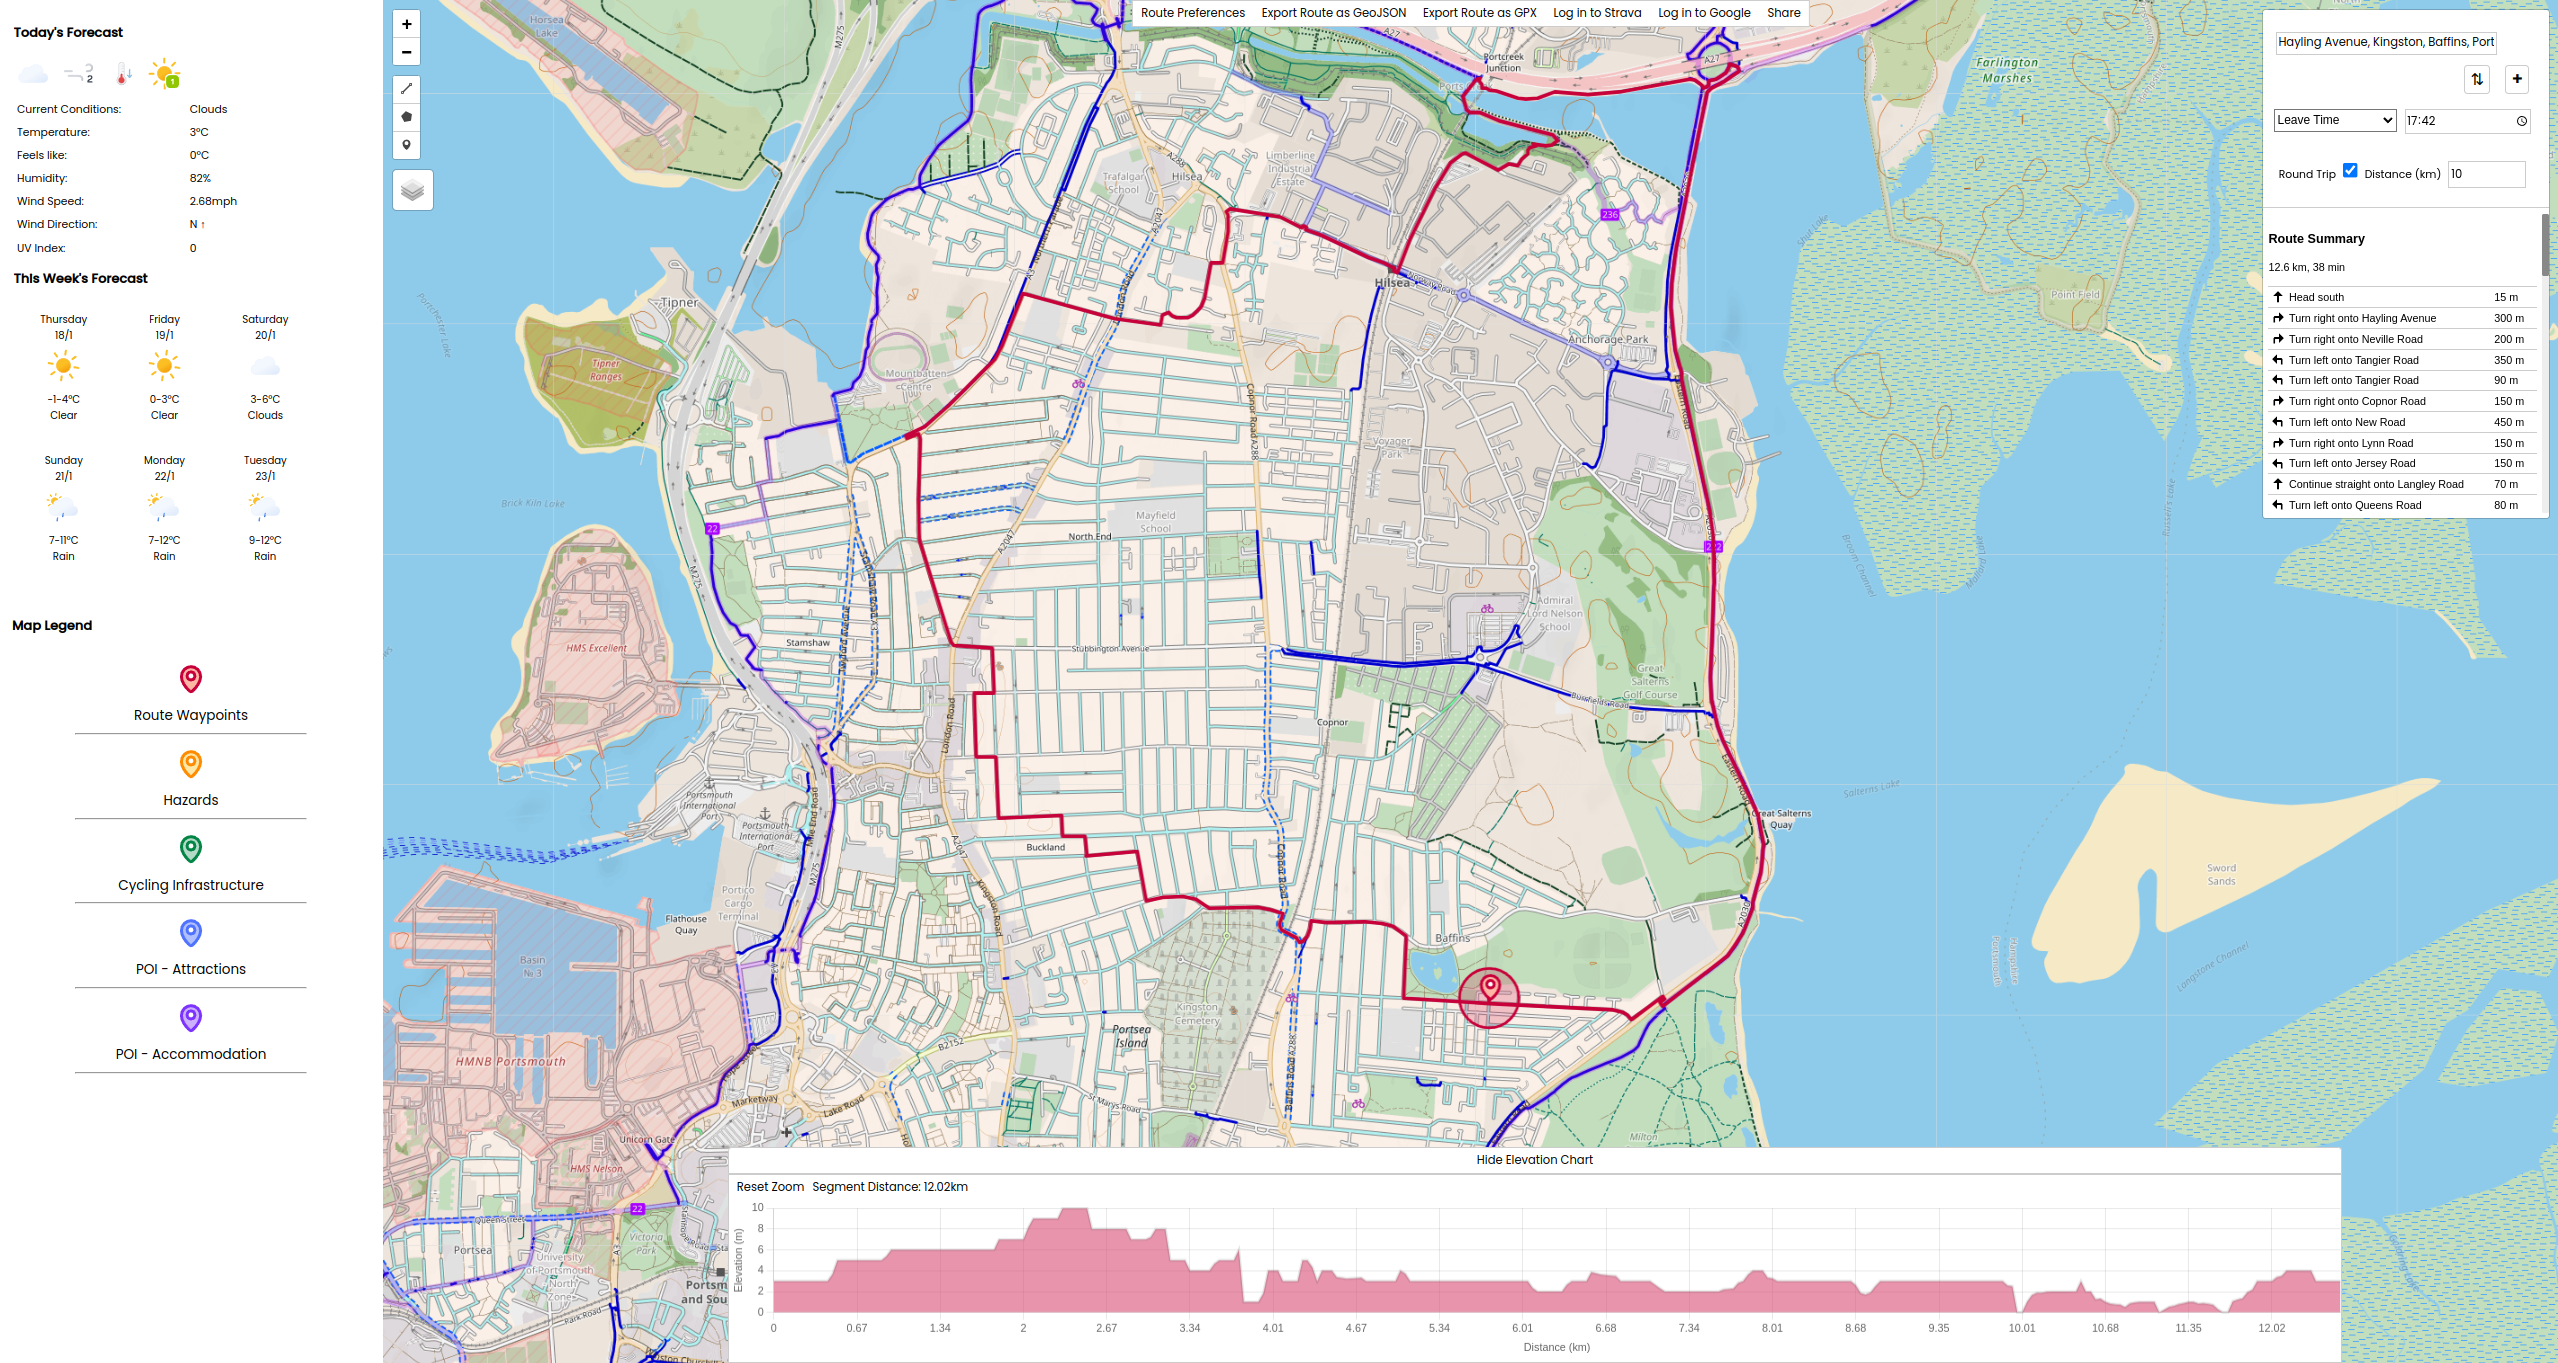
\includegraphics[width=425px]{figures/Progress Images/Iteration-3/SR11/SR11- Round Trip functionality working.png}
  \caption{Round Trip Route}
  \label{fig:round-trip}
\end{figure}

\subsection{Route Import}
\label{iteration3:route-import}

Importing routes was a vital feature as it would enable route sharing across many applications supporting the same standards. The GPX and GeoJSON file formats were chosen to be supported as they are the most common file formats used for route sharing and were already used for exporting routes from the artefact. Adding such a minor feature would enable the artefact to manually import routes from other applications, such as Strava, Komoot and RideWithGPS.

To interpret the GPX string, the DOMParser was used to parse the string into an XML document. The XML document was then traversed to find the route's latitude and longitude points, which were then stored in an array of latLng values. This array was then stored in a state variable called 'waypoints' whilst also being stored in LocalStorage. For GeoJSON, the JSON.parse method was used to parse the string, then the coordinates were extracted and stored in the same way as the coordinates in the GPX \see{fig:gpx-import}.

\begin{figure}[!ht]
  \centering
  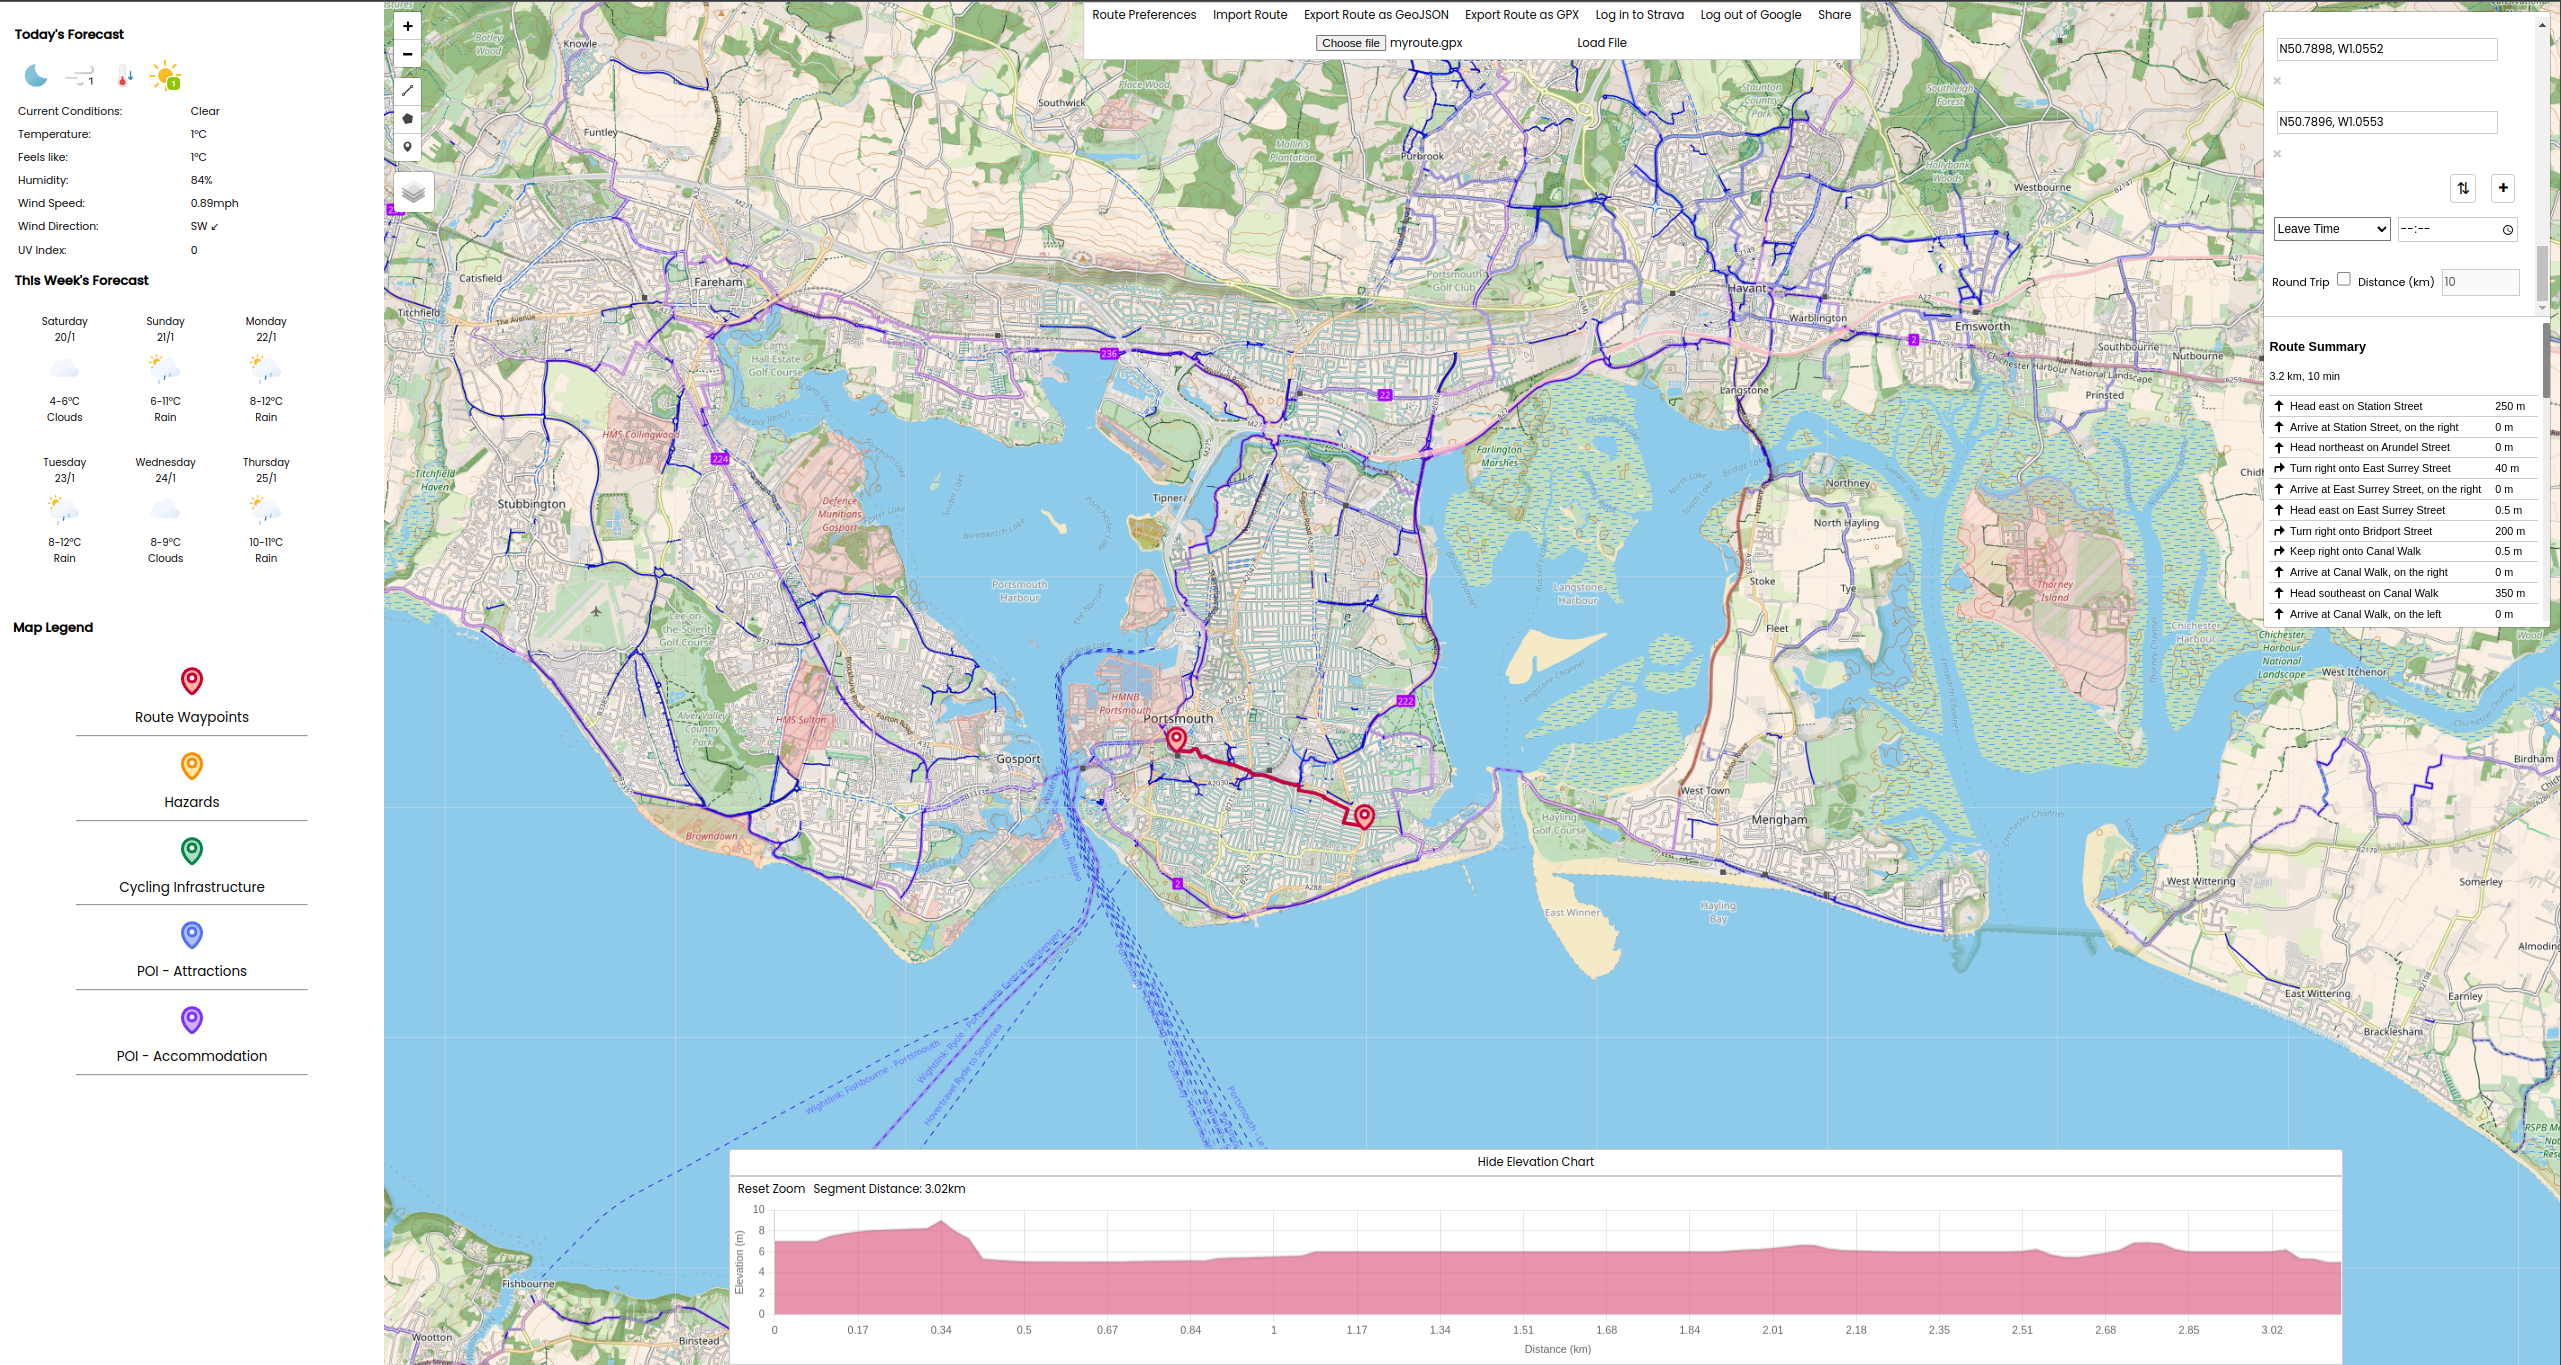
\includegraphics[width=425px]{figures/Progress Images/Iteration-3/SR48-49/SR48-Import GPX.png}
  \caption{Import GPX Route}
  \label{fig:gpx-import}
\end{figure}

\subsection{Garmin Connect Integration}
\label{iteration3:garmin-integration}

To integrate with the Garmin Connect API, the oAuth 1.0 protocol was implemented to allow the artefact to access the user's Garmin Connect account. The oAuth 1.0 protocol was implemented manually, as the Garmin Connect API documentation was clear on the oAuth process, having implemented oAuth 2.0 for Strava \see{iteration2:sharing-route}, the process was far easier to understand.

Once authentication had been completed, the create route endpoint was set up to handle the POST request from the frontend. The endpoint required the oAuth token, oAuth secret, the route details as a JSON string as per the Garmin documentation. The fetch API was then called to make the post request to the Go backend which would pass the route to the Garmin API to be uploaded. The route was then stored as a course in the user's Garmin Connect account, where it could be accessed from the Garmin Connect website or app \see{fig:garmin-connect}. 

\begin{figure}[!ht]
  \centering
  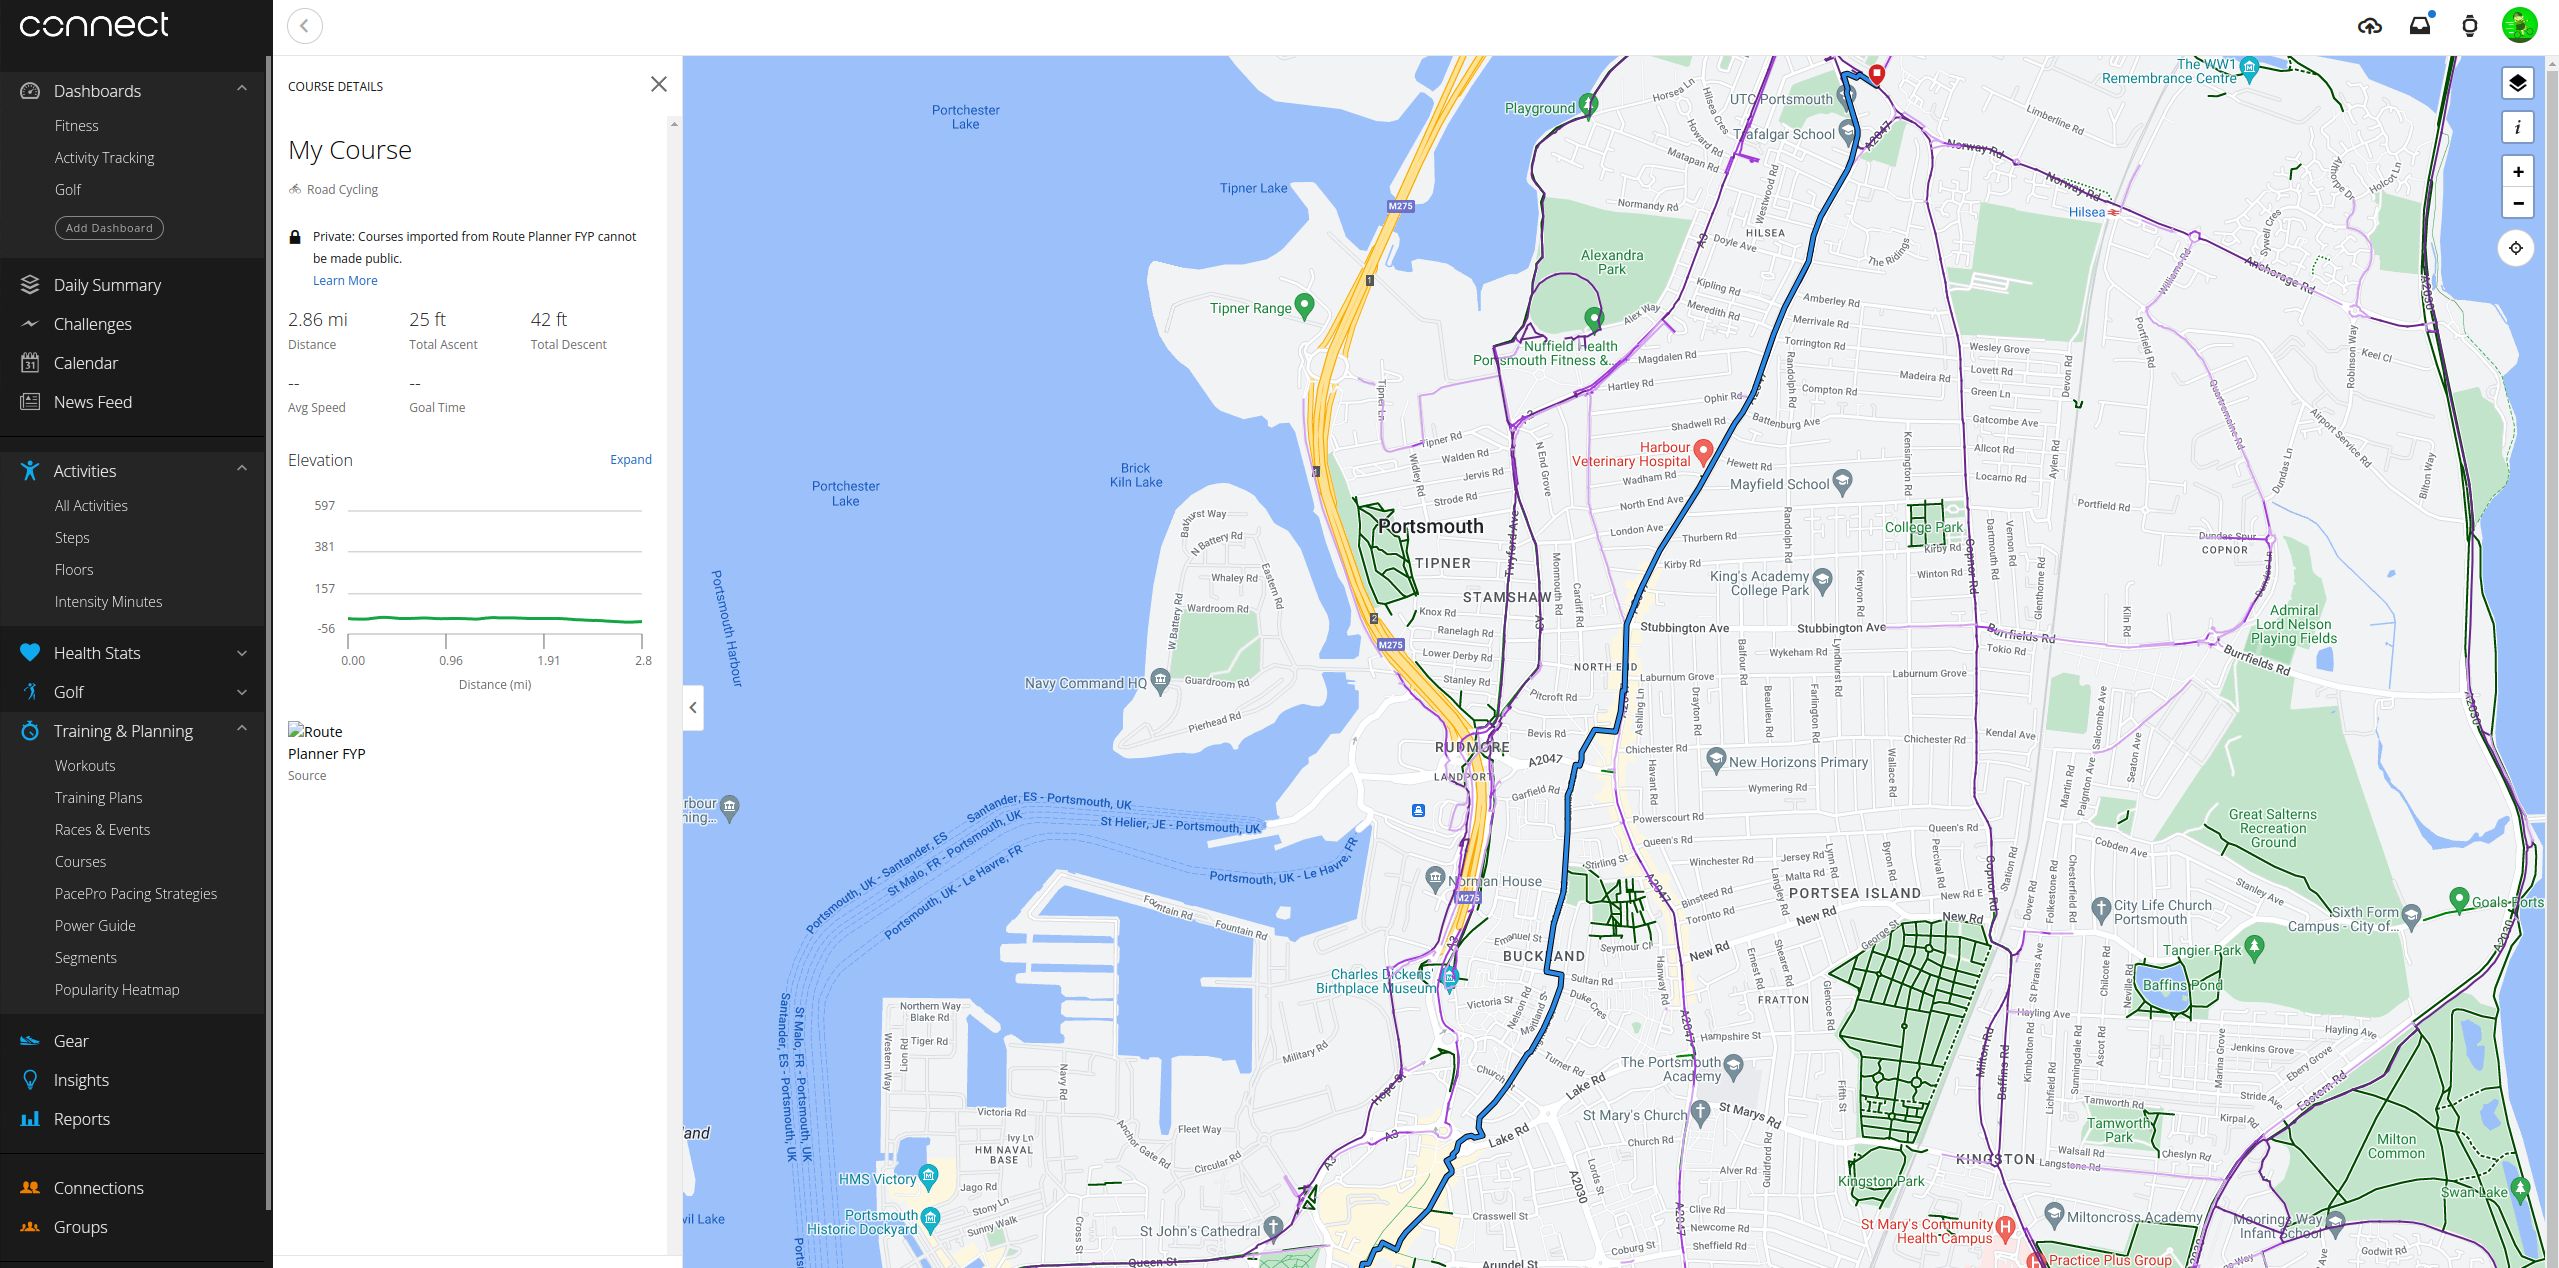
\includegraphics[width=425px]{figures/Progress Images/Iteration-3/SR50/SR50 - Garmin Connect App Course Viewer.png}
  \caption{Garmin Connect Successfully Uploaded Route}
  \label{fig:garmin-connect}
\end{figure}

\subsection{Social Media Sharing}
\label{iteration3:social-sharing}

The last feature to be implemented was social media sharing. The artefact was integrated with the Facebook, X(Twitter), and Reddit APIs to allow an image of the route to be shared to the user's social media account. To generate the image for sharing the leaflet screenshotter library was used (\cite{noauthor_leaflet-simple-map-screenshoter_2022}). The furthest two coordinates were calculated using the Euclidian distance formula \see{iteration3:euclidian-distance}, then the map's bounds were then set to fit the two points. The map was then screenshot and stored as a base64 string. This string was then passed to the respective social media API to be shared to the user's account \see{fig:facebook-share}.

\begin{equation}
  \label{iteration3:euclidian-distance}
  distance = \sqrt{(x_2 - x_1)^2 + (y_2 - y_1)^2}
\end{equation}
Where $x_1$ and $y_1$ are the latitude and longitude of the start point, and $x_2$ and $y_2$ are the latitude and longitude of the end point.

\begin{figure}[!ht]
  \centering
  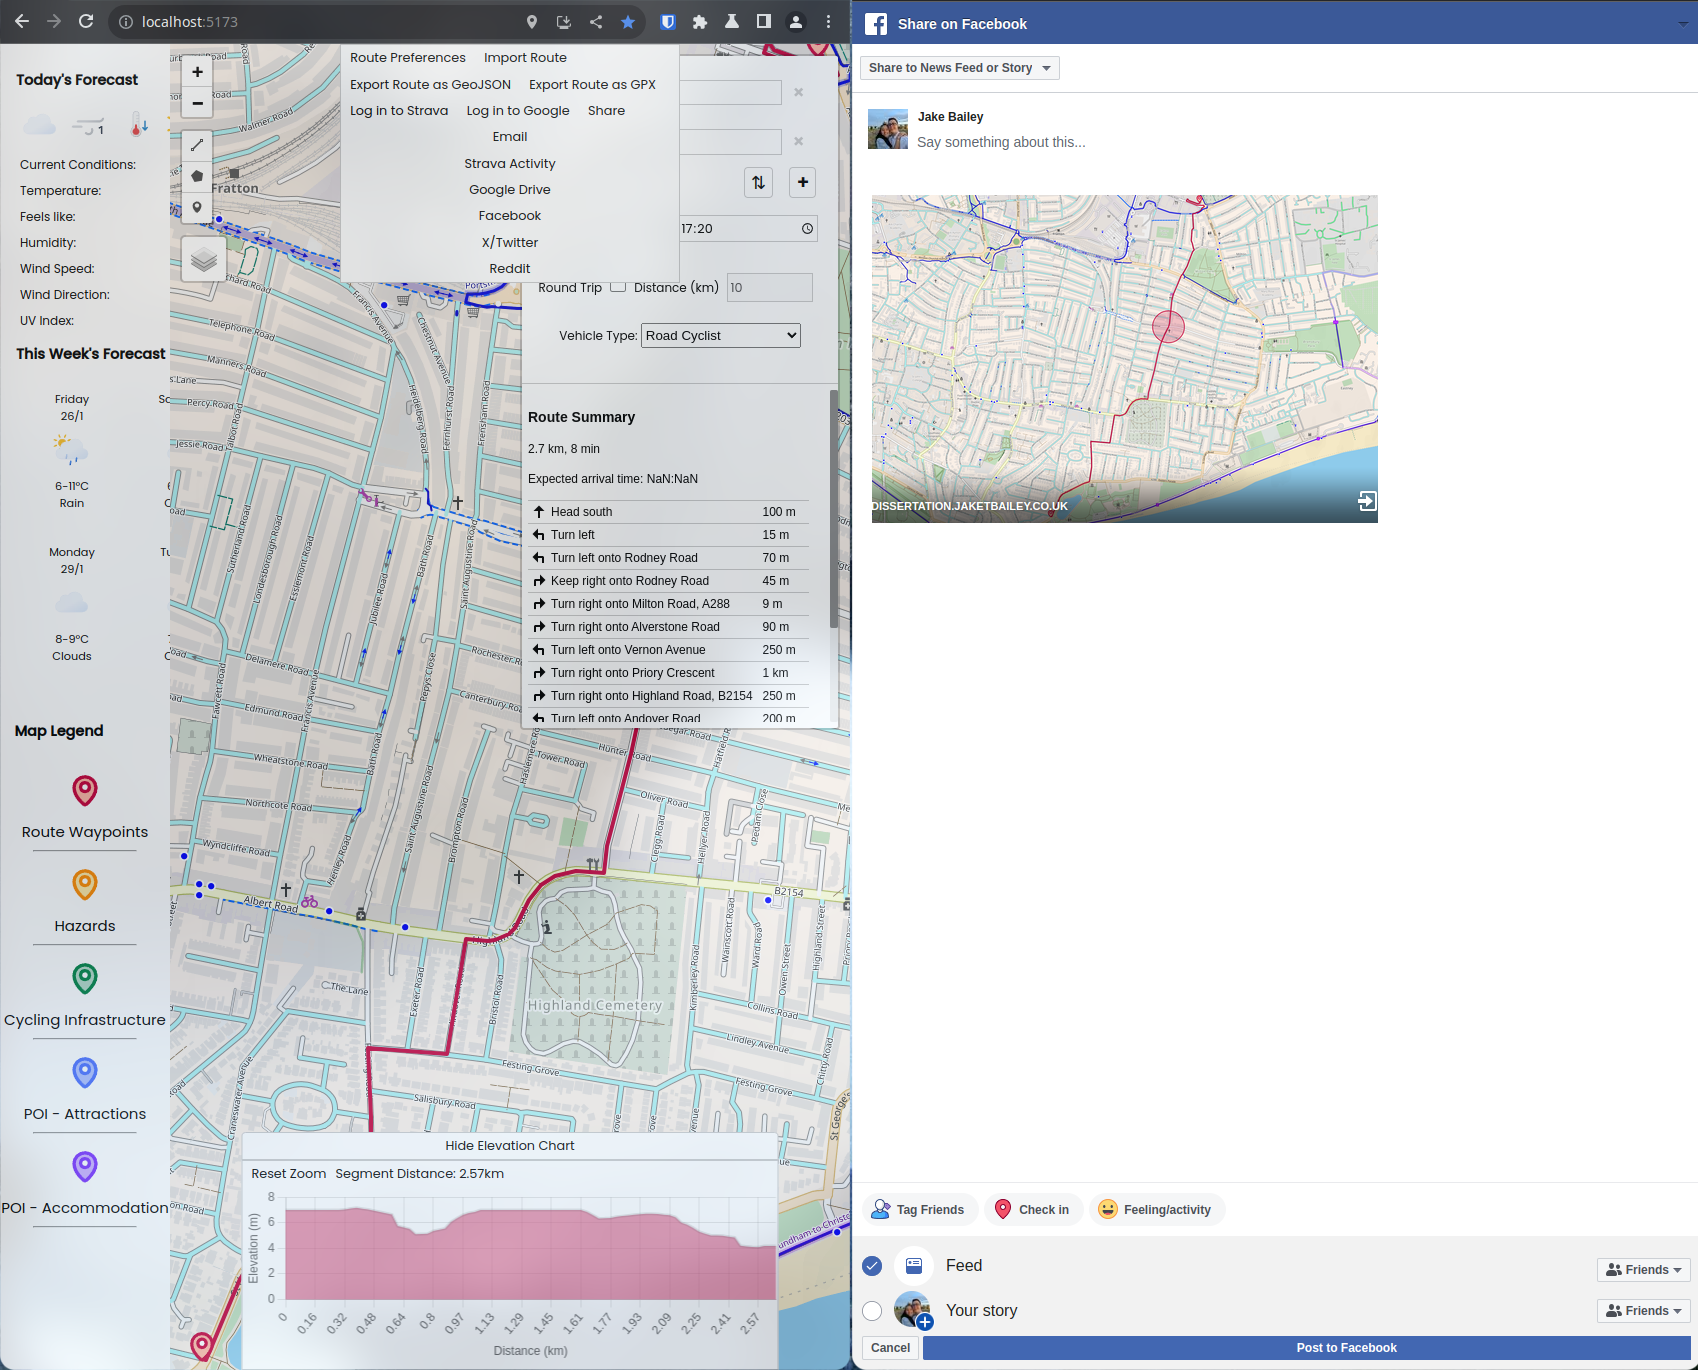
\includegraphics[width=425px]{figures/Progress Images/Iteration-3/SR51/SR51-Share to Facebook.png}
  \caption{Share to Facebook}
  \label{fig:facebook-share}
\end{figure}

\subsection{Main Challenges}
\label{iteration3:main-challenges}
